\documentclass{beamer}
\usepackage{listings}
\usepackage[font=footnotesize]{caption}
\usepackage[outdir=./images/]{epstopdf}
\epstopdfsetup{update}
\usepackage{float}
\usepackage{graphicx}
\usepackage{array}
\usepackage{lmodern}
\usepackage{varwidth}
\usepackage{amsmath}
\usepackage{tabularx}
\usepackage{adjustbox}
\usepackage{geometry}
\usepackage{color}
\definecolor{codegreen}{rgb}{0,0.6,0}
\definecolor{codegray}{rgb}{0.5,0.5,0.5}
\definecolor{codepurple}{rgb}{0.58,0,0.82}
\definecolor{backcolour}{rgb}{0.95,0.95,0.92}
\setbeamertemplate{footline}[frame number]

 \setbeamertemplate{footline}{%
        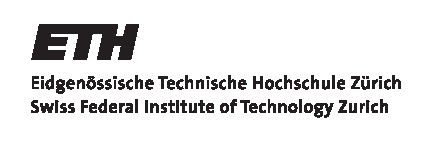
\includegraphics[height=0.5cm]{../figures/eth_logo_black.eps}%
	}


\lstdefinestyle{mystyle}{
	backgroundcolor=\color{backcolour},
	commentstyle=\color{codegreen},
	keywordstyle=\color{magenta},
	numberstyle=\tiny\color{codegray},
	stringstyle=\color{codepurple},
	basicstyle=\ttfamily\footnotesize,
	breakatwhitespace=false,
	breaklines=true,
	captionpos=b,
	keepspaces=true,
	numbers=left,
	numbersep=5pt,
	showspaces=false,
	showstringspaces=false,
	showtabs=false,
	tabsize=2
}
\lstset{style=mystyle}


\usetheme{Frankfurt}
\beamertemplatenavigationsymbolsempty

\title{On differentiable simulations of \\ haemodynamic systems}

\author{Diego Renner}

\begin{document}

\section{Introduction}
\maketitle

\begin{frame}
	\frametitle{Towards Personalised Medicine: Current Approaches}
	\begin{minipage}{0.59\textwidth}
		\begin{figure}[H]
			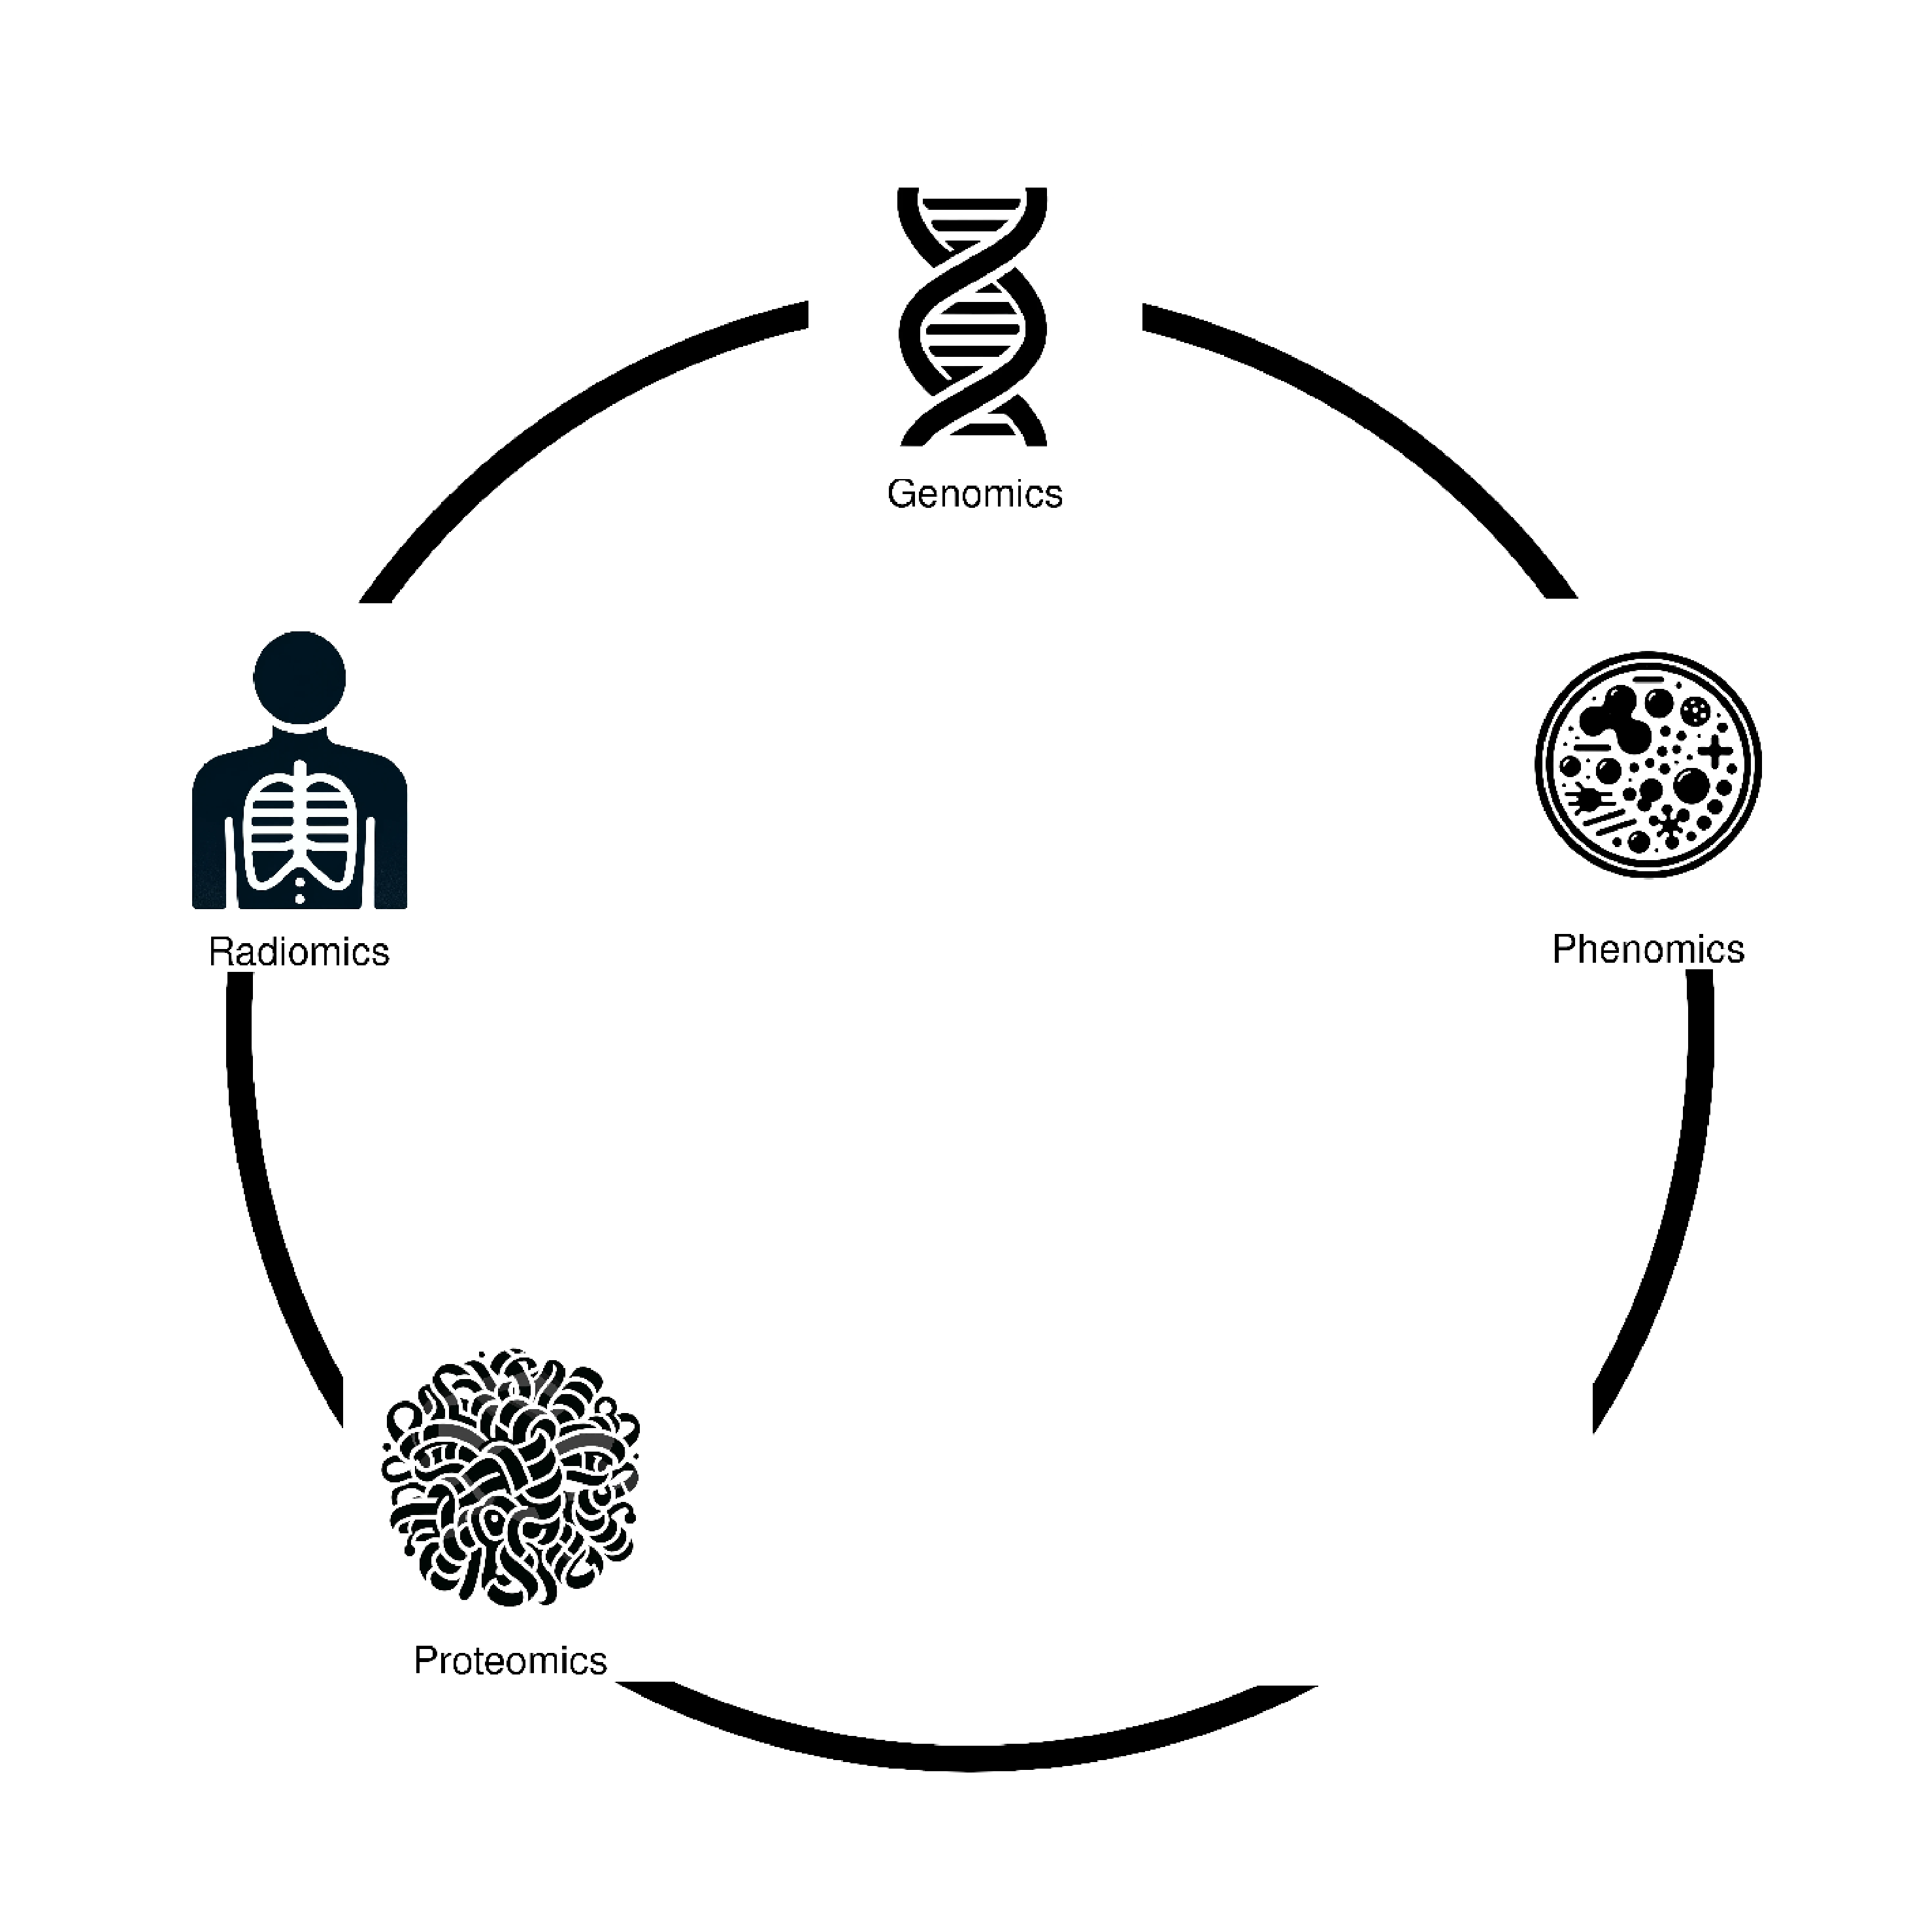
\includegraphics[width=\textwidth]{images/approaches_current.eps}
		\end{figure}
	\end{minipage} 
	\begin{minipage}{0.39\textwidth}
		\begin{minipage}[t][0.82\paperheight][t]{\textwidth}

		\end{minipage}
	\end{minipage}
\end{frame}
\begin{frame}
	\frametitle{Towards Personalised Medicine: Current Approaches}
	\begin{minipage}{0.59\textwidth}
		\begin{figure}[H]
			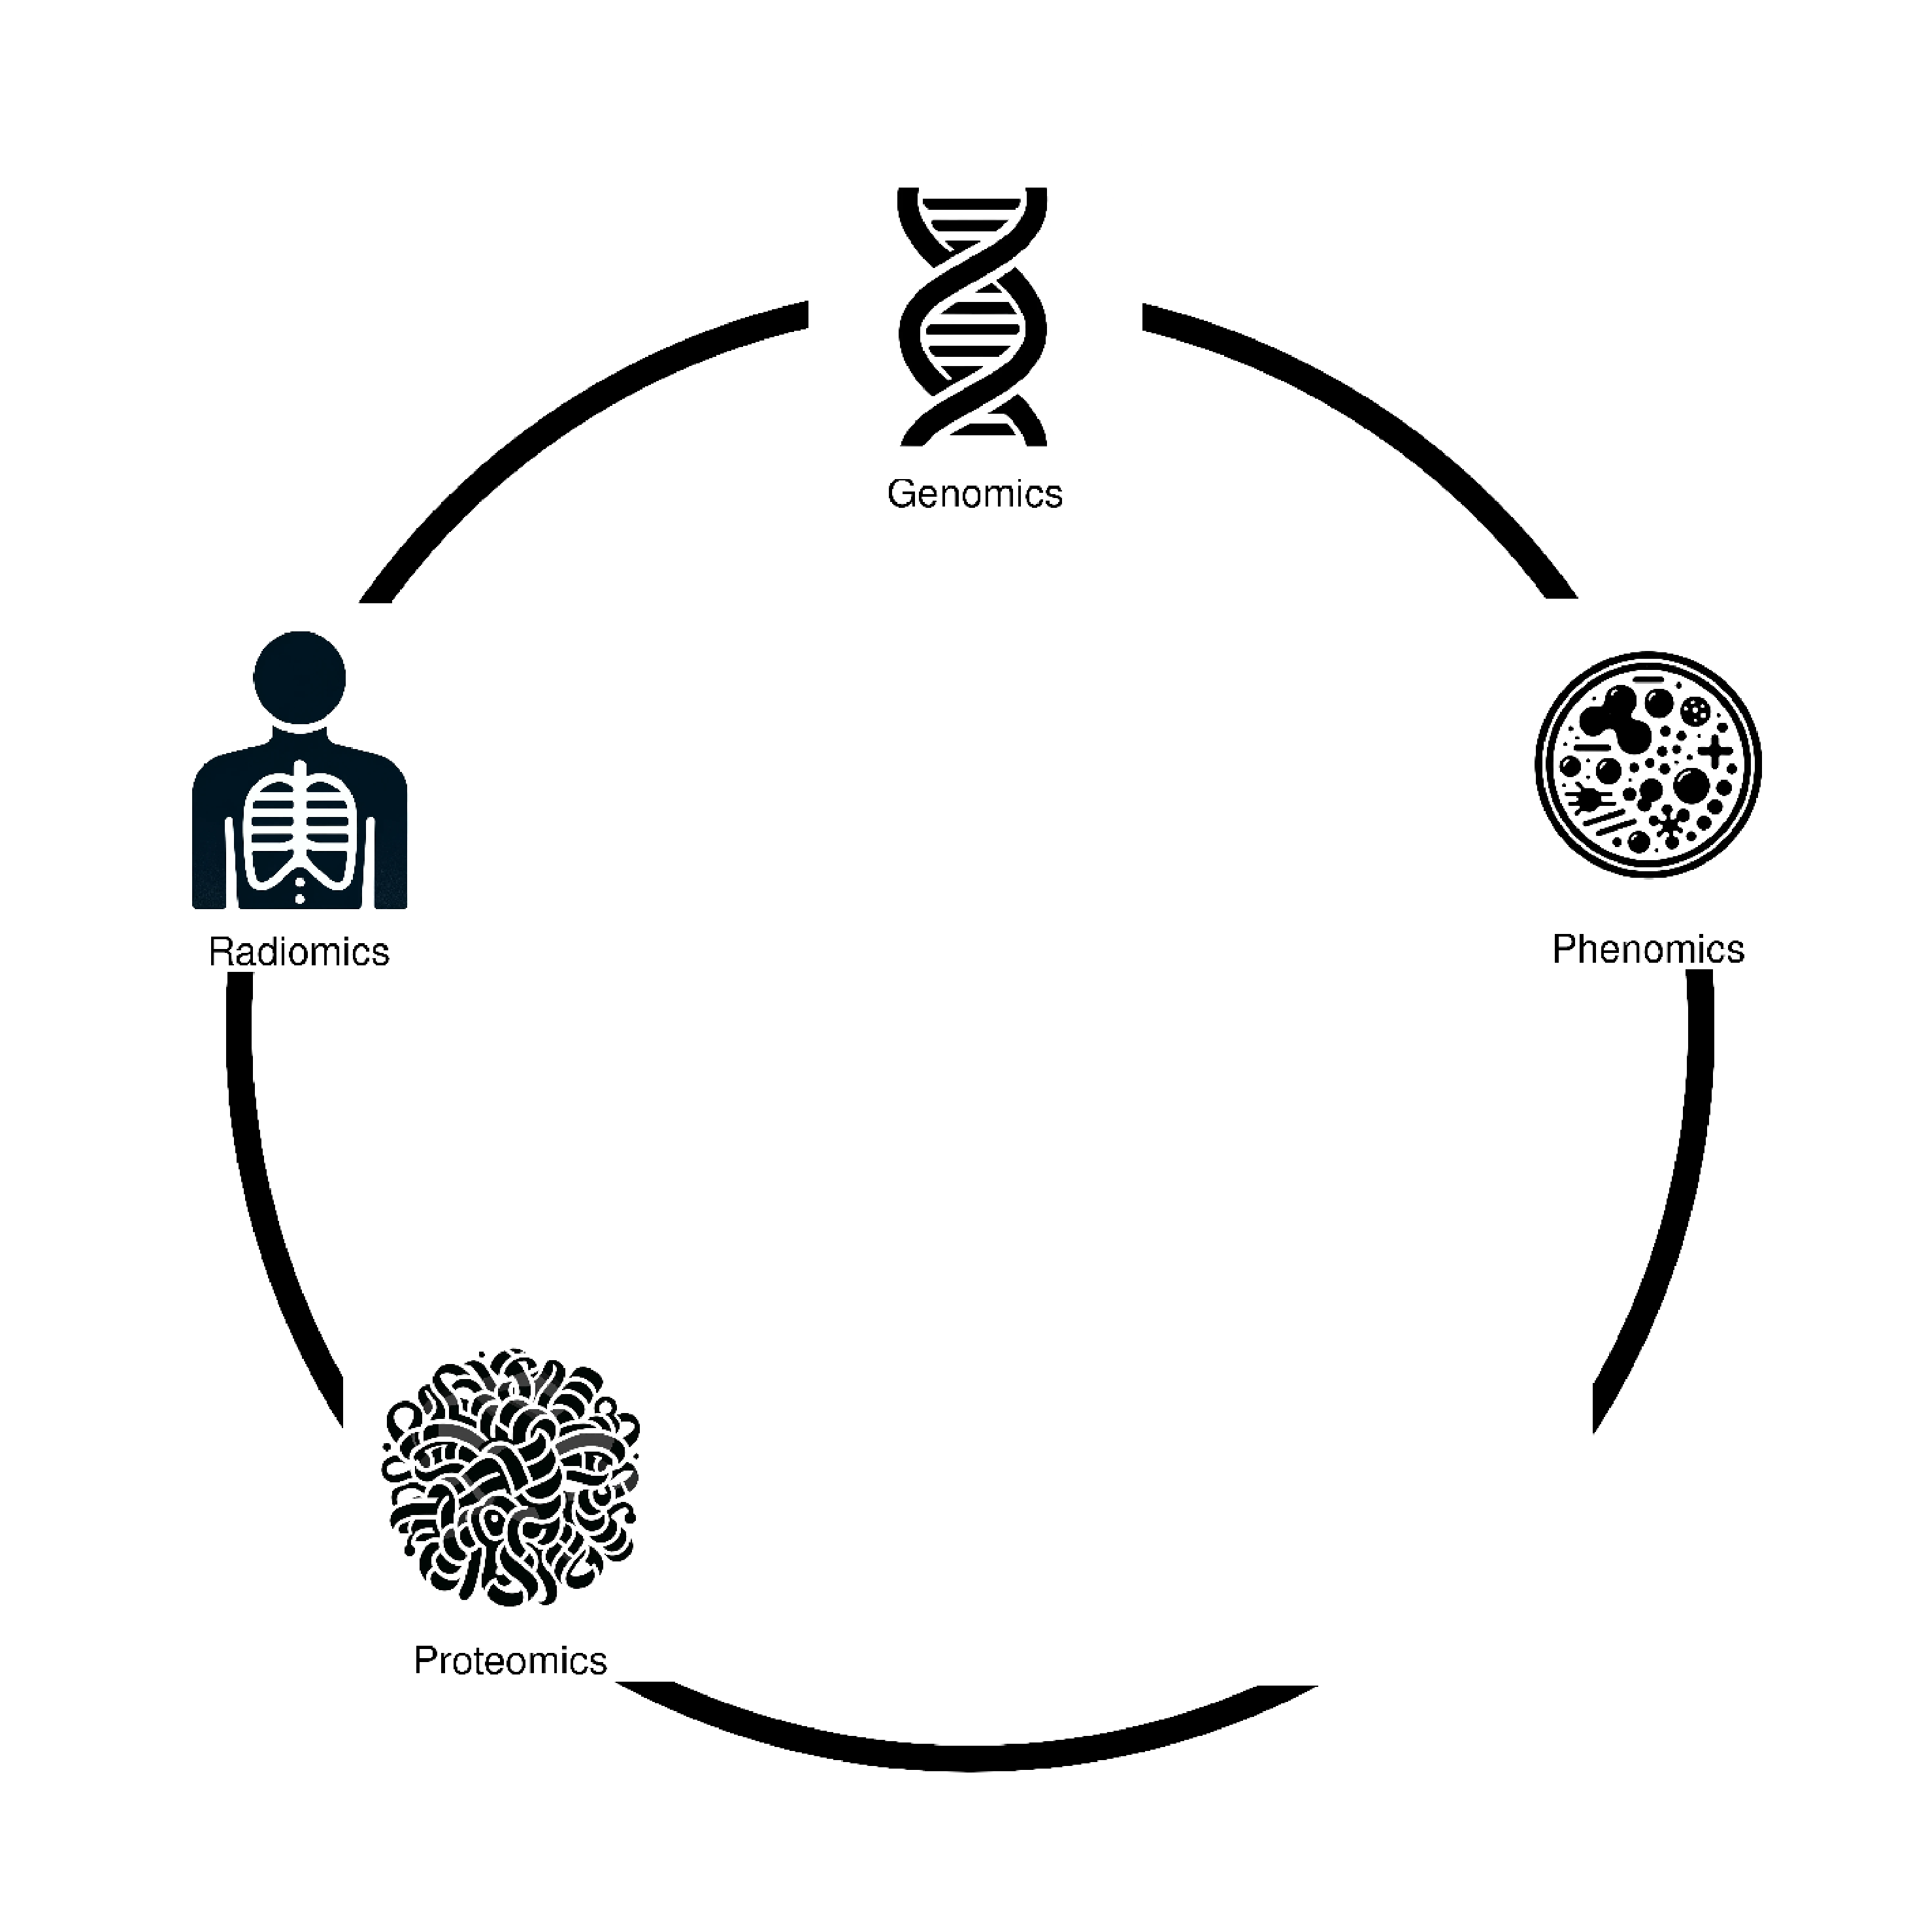
\includegraphics[width=\textwidth]{images/approaches_current.eps}
		\end{figure}
	\end{minipage} 
	\begin{minipage}{0.39\textwidth}
		\begin{minipage}[t][0.41\paperheight][t]{\textwidth}
			\begin{block}{Personalised Medicine}
				characterizing a patient and customizing their treatment according to which sub-population they fall into	
			\end{block}
		\end{minipage}
		\begin{minipage}[t][0.41\paperheight][t]{\textwidth}
		\end{minipage}
	\end{minipage}
\end{frame}
\begin{frame}
	\frametitle{Towards Personalised Medicine: Current Approaches}
	\begin{minipage}{0.59\textwidth}
		\begin{figure}[H]
			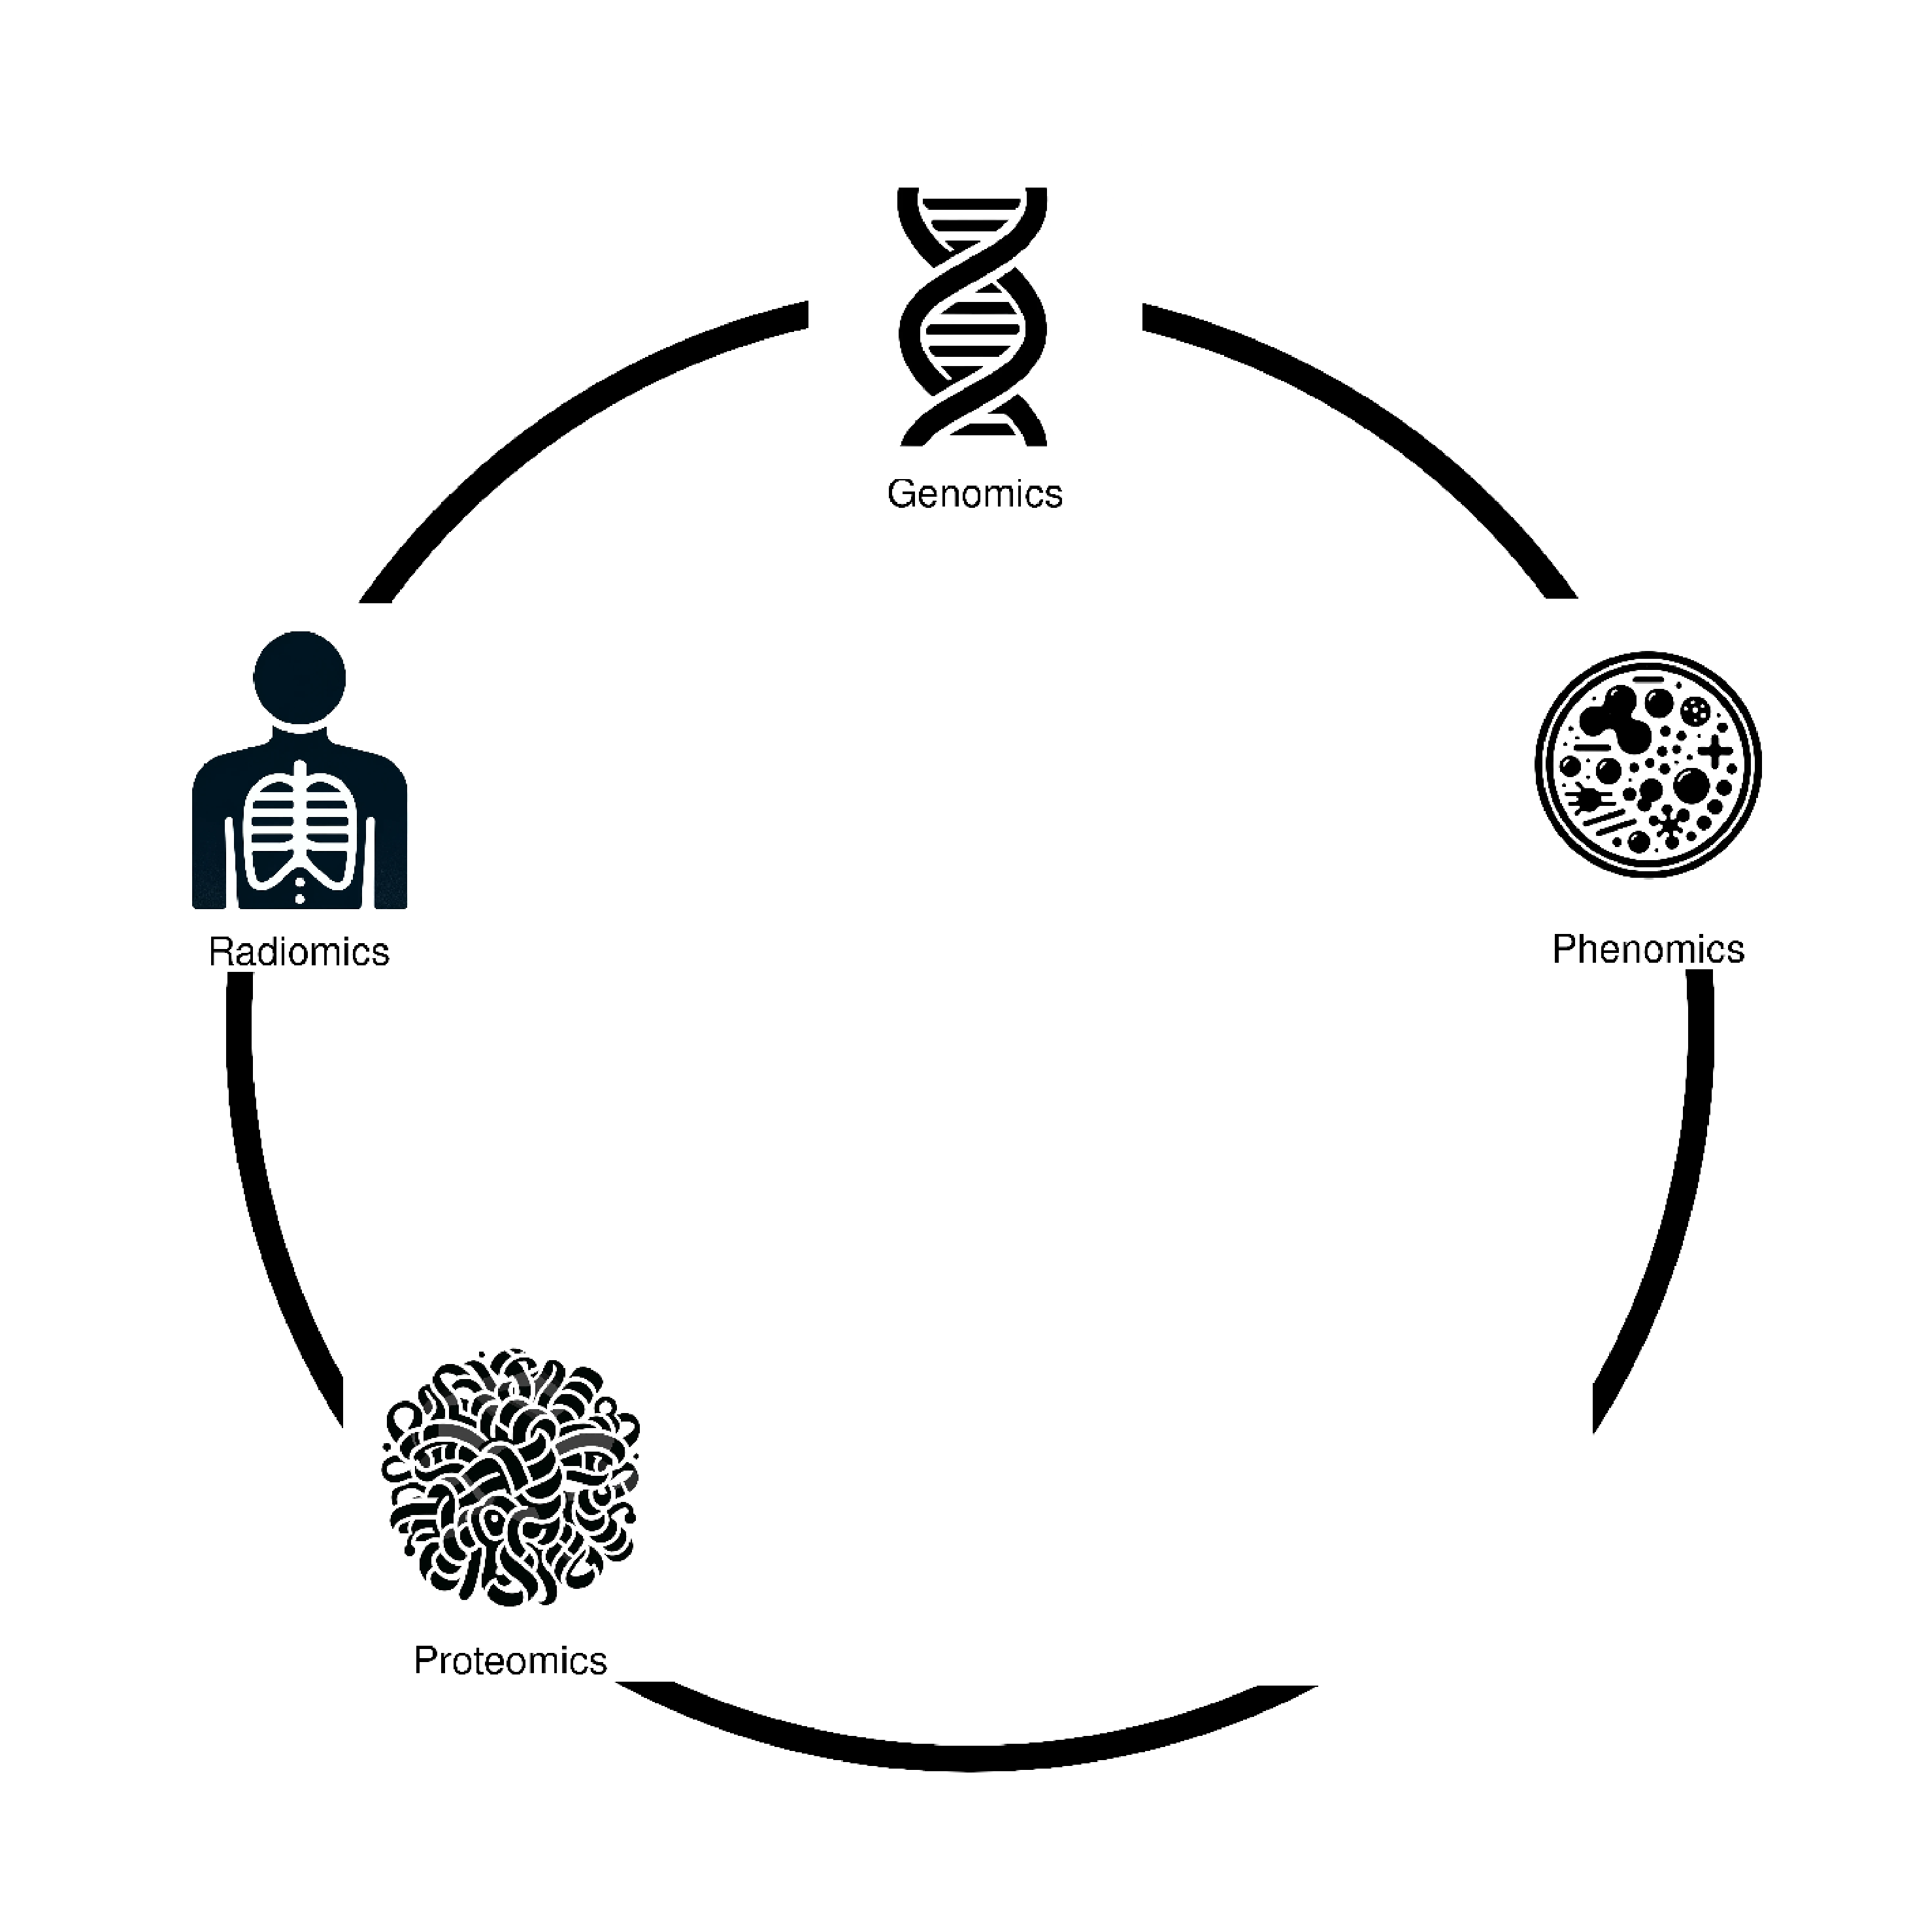
\includegraphics[width=\textwidth]{images/approaches_current.eps}
		\end{figure}
	\end{minipage} 
	\begin{minipage}{0.39\textwidth}
		\begin{minipage}[t][0.41\paperheight][t]{\textwidth}
			\begin{block}{Personalised Medicine}
				characterizing a patient and customizing their treatment according to which sub-population they fall into	
			\end{block}
		\end{minipage}
		\begin{minipage}[t][0.41\paperheight][t]{\textwidth}
			\begin{block}{Biomarkers}
				measurable quantities that can aid in diagnosis and treatment of a disease
			\end{block}
		\end{minipage}
	\end{minipage}
\end{frame}

\begin{frame}
	\frametitle{Towards Personalised Medicine: Future Approaches}
	\begin{minipage}{0.59\textwidth}
		\begin{figure}[H]
			\includegraphics[width=\textwidth]{images/approaches_future.eps}
		\end{figure}
	\end{minipage} \hfill
	\begin{minipage}[T][0.82\paperheight][T]{0.39\textwidth}
	\end{minipage}
\end{frame}
\begin{frame}
	\frametitle{Towards Personalised Medicine: Future Approaches}
	\begin{minipage}{0.59\textwidth}
		\begin{figure}[H]
			\includegraphics[width=\textwidth]{images/approaches_future.eps}
		\end{figure}
	\end{minipage} \hfill
	\begin{minipage}{0.39\textwidth}
		\begin{minipage}[t][0.56\paperheight][t]{\textwidth}
			\begin{block}{Model Based Approach}
				use patient specific parameters to setup well-defined computational models that output biomarkers which are strongly and causally related to the occurrence or the outcome of a disease
			\end{block}
		\end{minipage}
		\begin{minipage}[t][0.26\paperheight][t]{\textwidth}
		\end{minipage}
	\end{minipage}
\end{frame}
\begin{frame}
	\frametitle{Towards Personalised Medicine: Future Approaches}
	\begin{minipage}{0.59\textwidth}
		\begin{figure}[H]
			\includegraphics[width=\textwidth]{images/approaches_future.eps}
		\end{figure}
	\end{minipage} \hfill
	\begin{minipage}{0.39\textwidth}
		\begin{minipage}[t][0.56\paperheight][t]{\textwidth}
			\begin{block}{Model Based Approach}
				use patient specific parameters to setup well-defined computational models that output biomarkers which are strongly and causally related to the occurrence or the outcome of a disease
			\end{block}
		\end{minipage}
		\begin{minipage}[t][0.26\paperheight][t]{\textwidth}
			\begin{block}{Example}
				$\hookrightarrow$
			\end{block}
		\end{minipage}
	\end{minipage}
\end{frame}
\begin{frame}<1>[label=ph]
	\frametitle{Example: Pulmonary Hypertension (PH)}
	\begin{itemize}
		\item<1-> affect large parts of the population
		\item<2-> heavily studied but currently no perfect solution 
		\item<3-> \begin{tabularx}{\linewidth}{| >{\centering\arraybackslash}m{0.4\linewidth} | >{\centering\arraybackslash}m{0.25\linewidth} | >{\centering\arraybackslash}X |} 
				\hline
				biomarker(s) & measurement & correlation \\ 
				\hline
				\hline
				absolute vascular pressure & invasive & strong \\ 
				\hline
				brain natriuretic peptide & blood sampling & weaker \\ 
				\hline
			\end{tabularx}
		\item<4->
			$\Rightarrow$ accurately determining the absolute vascular pressure through a computational model would allow reliable prognosis of PH while avoiding the risk of an invasive procedure
		\item<5-> problem: need patient specific parameters for model
	\end{itemize}
\end{frame}

\againframe<2>{ph}
\againframe<3>{ph}
\againframe<4>{ph}
\againframe<5>{ph}

\section{Model Pipeline}
\begin{frame}<1>[label=mp]
	\only<1-2>{\frametitle{3D Model Pipeline}}
	\only<3-99>{\frametitle{1D Model Pipeline}}
	\only<100->{\frametitle{Parameter Inference Pipeline}}
	\vspace{-10pt}
	\begin{figure}[htbp]
		\only<-99>{\begin{minipage}[t][0.06\paperheight][t]{\linewidth}
			\begin{minipage}{0.18\linewidth}
				\caption*{\tiny Medical Imaging}
			\end{minipage}
			\hfill
			\begin{minipage}{0.1\linewidth}
				\caption*{\tiny}
			\end{minipage}
			\hfill
			\begin{minipage}{0.18\linewidth}
				\caption*{\tiny 3D Geometry}
			\end{minipage}
			\hfill
			\begin{minipage}{0.1\linewidth}
				\caption*{\tiny}
			\end{minipage}
			\hfill
			\only<1-2>{\begin{minipage}{0.18\linewidth}
				\caption*{\tiny}
		\end{minipage}}
			\only<3->{\begin{minipage}{0.18\linewidth}
				\caption*{\tiny 1D Geometry}
		\end{minipage}}
			\hfill
			\begin{minipage}{0.1\linewidth}
				\caption*{\tiny}
			\end{minipage}
		\end{minipage}
		\begin{minipage}[c][0.33\paperheight][c]{\linewidth}
			\begin{minipage}{0.18\linewidth}
				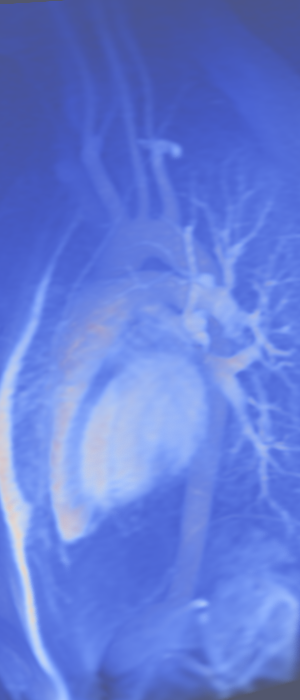
\includegraphics[width=\linewidth]{images/medical_imaging_0007.eps}
			\end{minipage}
			\hfill
			\begin{minipage}{0.1\linewidth}
				
\includegraphics[width=\linewidth]{images/right_arrow.png}
			\end{minipage}
			\hfill
			\begin{minipage}{0.18\linewidth}
				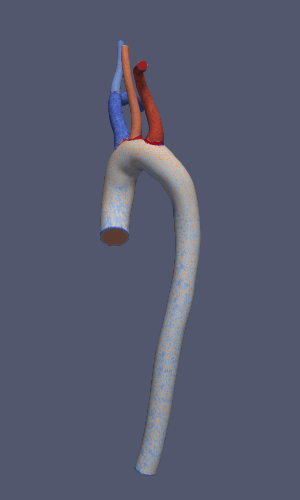
\includegraphics[width=\linewidth]{images/3d_model_0007.eps}
			\end{minipage}
			\hfill
			\begin{minipage}{0.1\linewidth}
				
\includegraphics[width=\linewidth]{images/right_arrow.png}
			\end{minipage}
			\hfill
			\only<1-2>{\begin{minipage}{0.18\linewidth}
				{\huge \hfill .\hfill .\hfill .}
		\end{minipage}}
			\only<3->{\begin{minipage}{0.18\linewidth}
				\includegraphics[width=\linewidth]{images/1d_model_0007.eps}
		\end{minipage}}
			\hfill
			\begin{minipage}{0.1\linewidth}
				
\includegraphics[width=\linewidth]{images/right_arrow.png}
			\end{minipage}
	\end{minipage}}
	\only<100>{
		\begin{minipage}[t][0.06\paperheight][t]{\linewidth}
			\begin{minipage}{0.1\linewidth}
				\caption*{\tiny}
			\end{minipage}
			\hfill
			\begin{minipage}{0.58\linewidth}
				\caption*{\tiny Parameter Inference}
			\end{minipage}
			\hfill
			\begin{minipage}{0.1\linewidth}
				\caption*{\tiny }
			\end{minipage}
		\end{minipage}
		\begin{minipage}[c][0.35\paperheight][c]{\linewidth}
			\begin{minipage}{0.1\linewidth}
				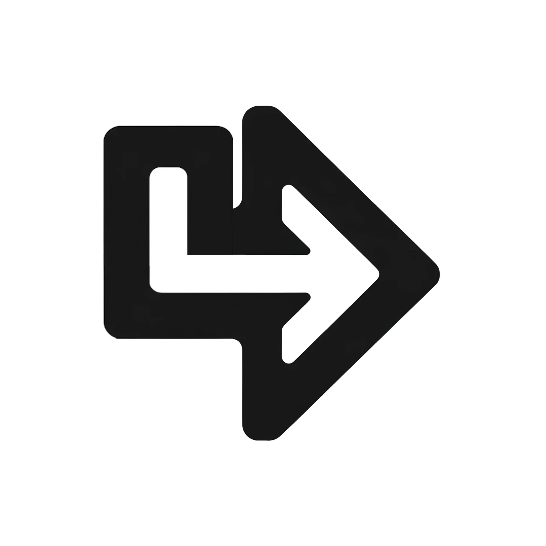
\includegraphics[angle=270, width=\linewidth]{images/left_turn_arrow.eps}
			\end{minipage}
			\hfill
			\begin{minipage}{0.58\linewidth}
				{\footnotesize \begin{itemize} 
					\item MCMC \& gradient information $\rightarrow$ Hamiltionian Monte Carlo (HMC)
					\item HMC \& adaptively setting path length $\rightarrow$ No-U-Turn Sampler (NUTS)
					\item Provided by Numpyro
			\end{itemize}}
			\end{minipage}
			\hfill
			\begin{minipage}{0.1\linewidth}
				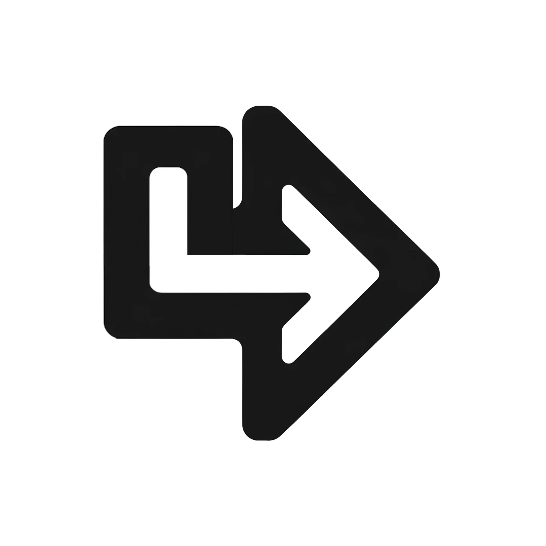
\includegraphics[angle=180, width=\linewidth]{images/left_turn_arrow.eps}
			\end{minipage}
	\end{minipage}}
		\vfill
		\begin{minipage}[t][0.06\paperheight][t]{\linewidth}
			\begin{minipage}{0.18\linewidth}
				\caption*{\tiny Parameters}
			\end{minipage}
			\hfill
			\begin{minipage}{0.1\linewidth}
				\caption*{\tiny}
			\end{minipage}
			\hfill
			\begin{minipage}{0.18\linewidth}
				\caption*{\tiny Solver}
			\end{minipage}
			\hfill
			\begin{minipage}{0.1\linewidth}
				\caption*{\tiny}
			\end{minipage}
			\hfill
			\begin{minipage}{0.18\linewidth}
				\caption*{\tiny Biomarkers}
			\end{minipage}
			\hfill
			\begin{minipage}{0.1\linewidth}
				\caption*{\tiny}
			\end{minipage}
		\end{minipage}
		\begin{minipage}[c][0.33\paperheight][c]{\linewidth}
			\begin{minipage}{0.18\linewidth}
				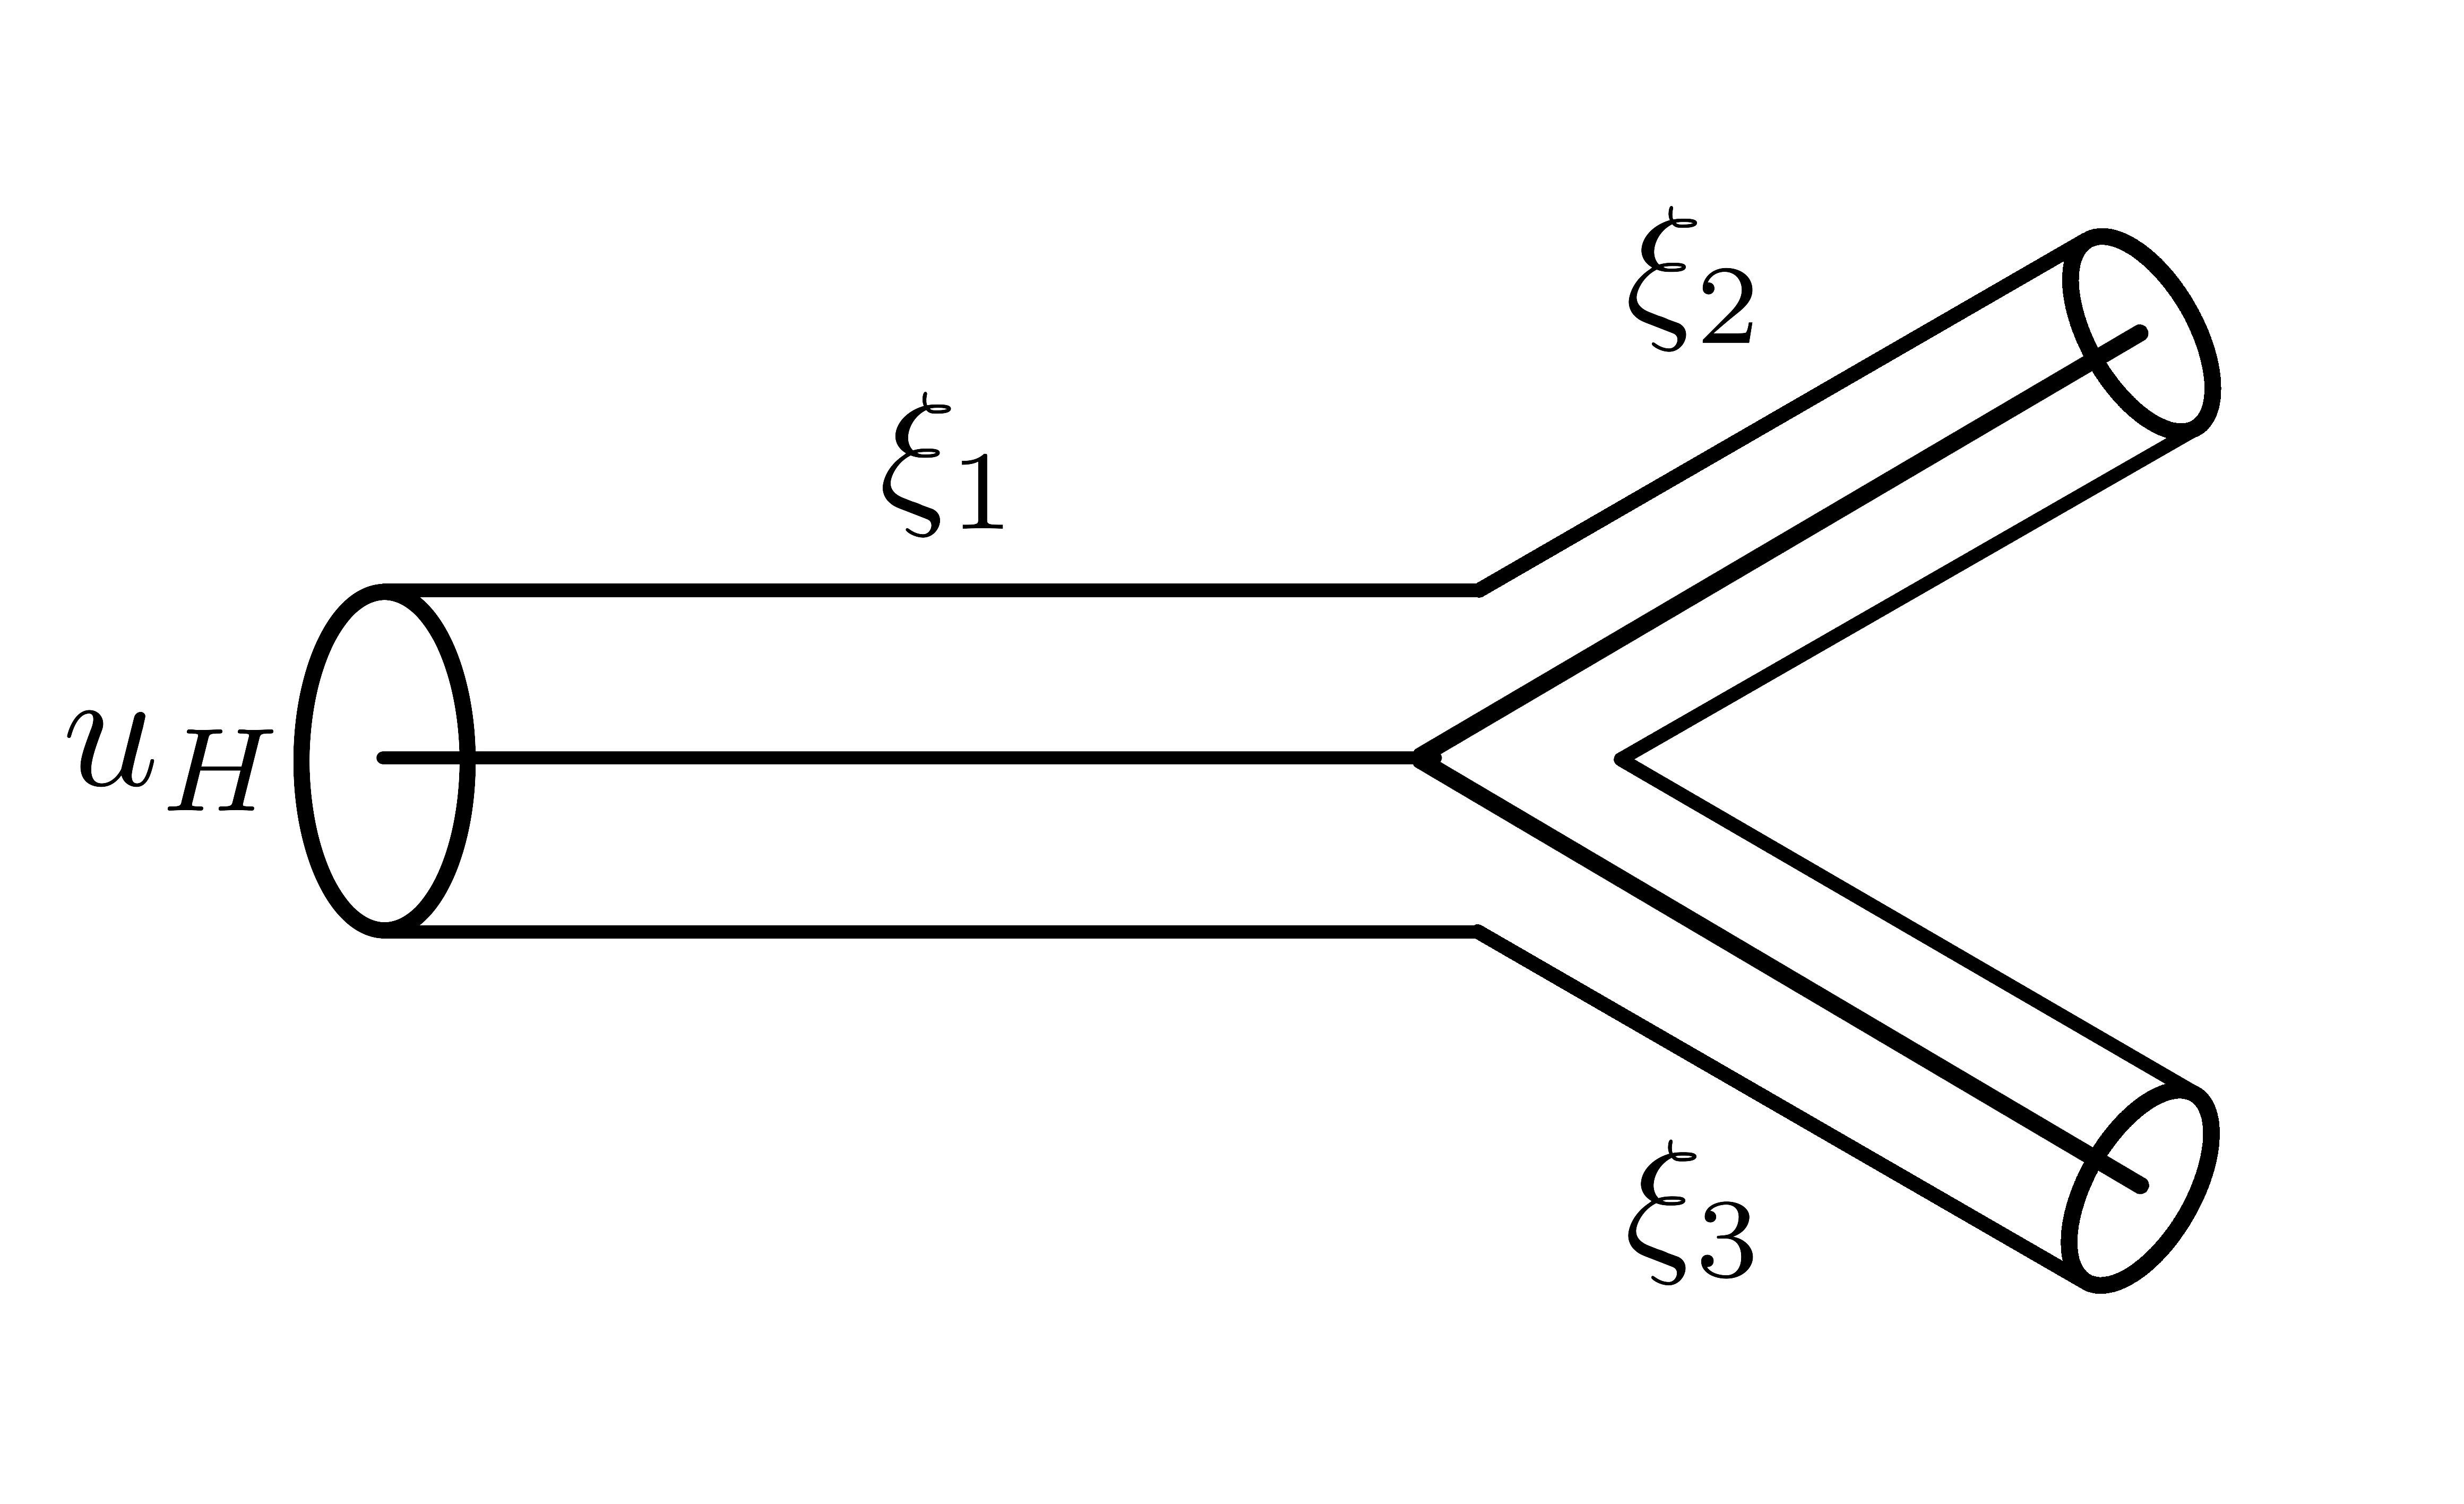
\includegraphics[width=\linewidth]{images/bifurcation.eps}
			\end{minipage}
			\hfill
			\begin{minipage}{0.1\linewidth}
				
\includegraphics[width=\linewidth]{images/right_arrow.png}
			\end{minipage}
			\hfill
			\begin{minipage}{0.18\linewidth}
				{\tiny
					\begin{itemize} 
						\item fluid 
						\item structure 
						\item fluid-structure
				\end{itemize}}
		\end{minipage}
			\hfill
			\begin{minipage}{0.1\linewidth}
				
\includegraphics[width=\linewidth]{images/right_arrow.png}
			\end{minipage}
			\hfill
			\only<1-2>{\begin{minipage}{0.18\linewidth}
				\includegraphics[width=\linewidth]{images/3d_biomarkers_0007.eps}
		\end{minipage}}
		\only<3->{\begin{minipage}{0.18\linewidth}
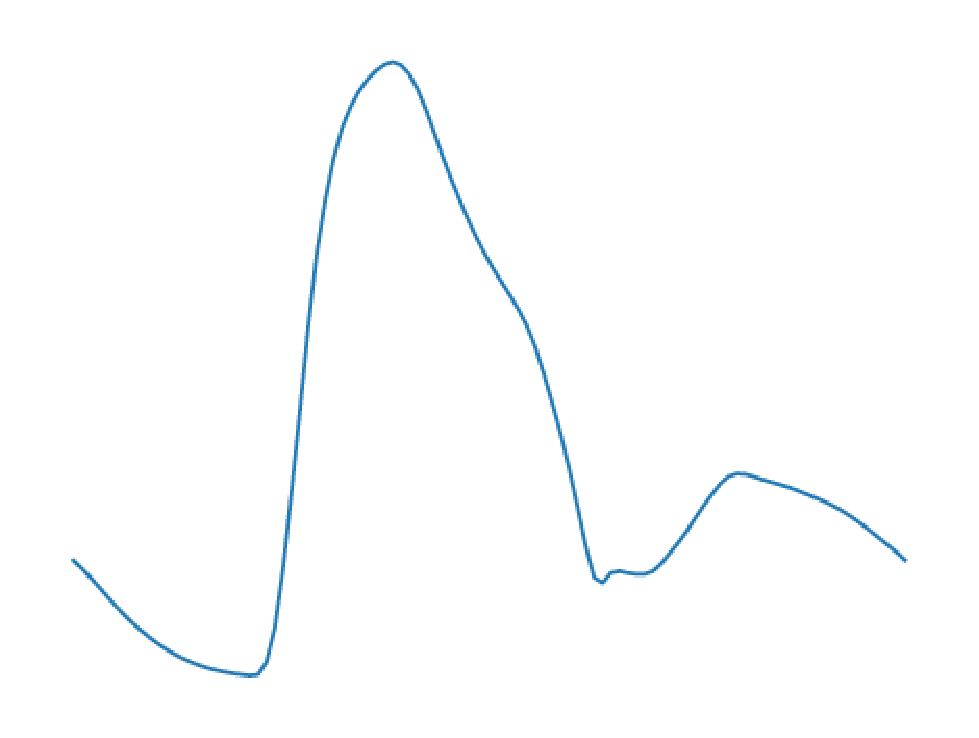
\includegraphics[width=\linewidth]{images/adan56_tibiofibular_trunk_L_P.eps}
		\end{minipage}}
		\hfill
			\only<2>{\begin{minipage}{0.1\linewidth}
				\caption*{\color{red} too expensive!}
		\end{minipage}}
		\hfill
		\only<3-99>{\begin{minipage}{0.1\linewidth}
			\caption*{\tiny}
	\end{minipage}}
		\only<100>{\begin{minipage}{0.1\linewidth}
				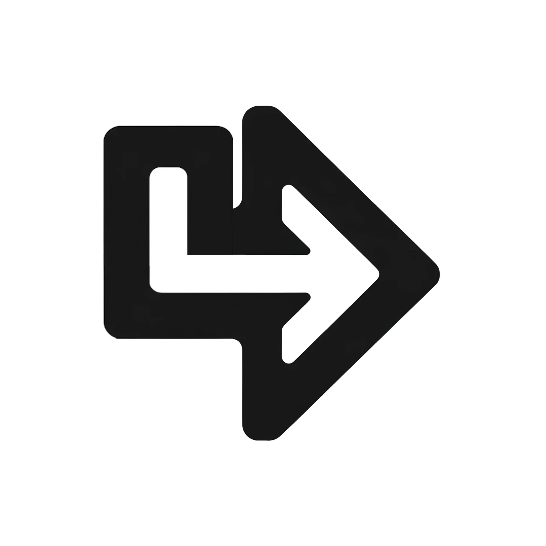
\includegraphics[angle=90, width=\linewidth]{images/left_turn_arrow.eps}
	\end{minipage}}
		\end{minipage}
	\end{figure}
\end{frame}

\againframe<2>{mp}
\againframe<3>{mp}

\begin{frame}[label=1dge]
	\frametitle{1D Geometry Extraction: Slicer 3D + VMTK}
		\begin{minipage}{\linewidth}
			\onslide<1->{\begin{minipage}{0.25\linewidth}
				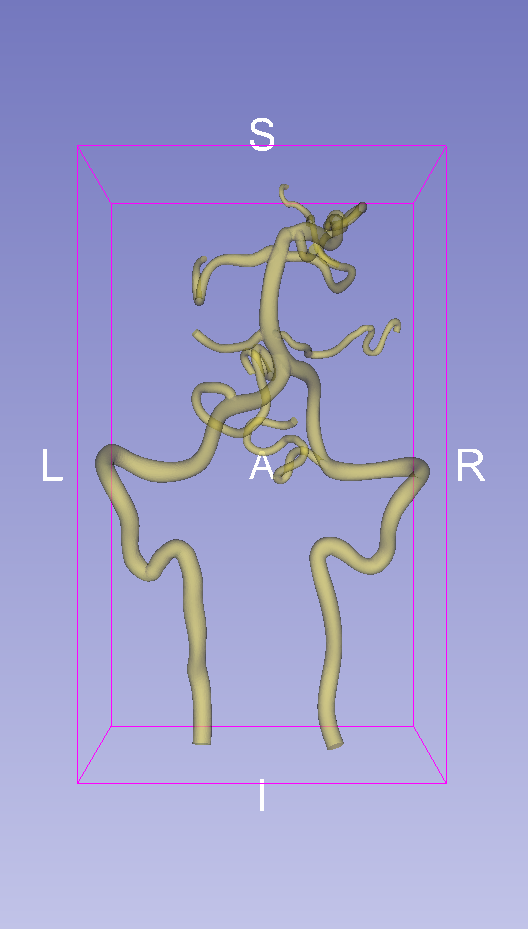
\includegraphics[width=\linewidth]{images/0053_extract1.png}
		\end{minipage}}
			\onslide<3->{\begin{minipage}{0.1\linewidth}
				\scalebox{-1}[1]{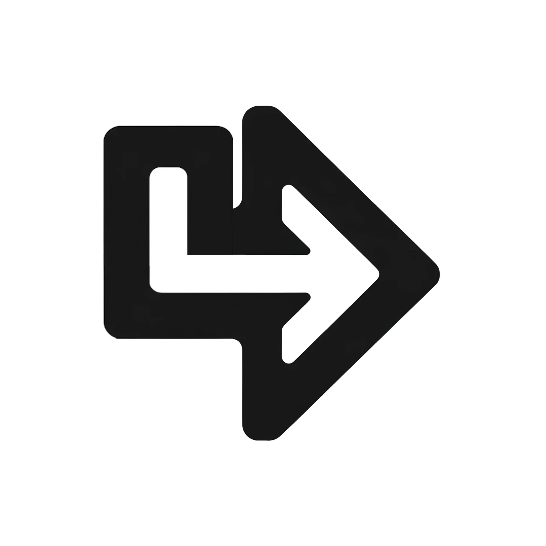
\includegraphics[width=\linewidth, angle=180]{images/left_turn_arrow.eps}}
		\end{minipage}
			\begin{minipage}{0.25\linewidth}
				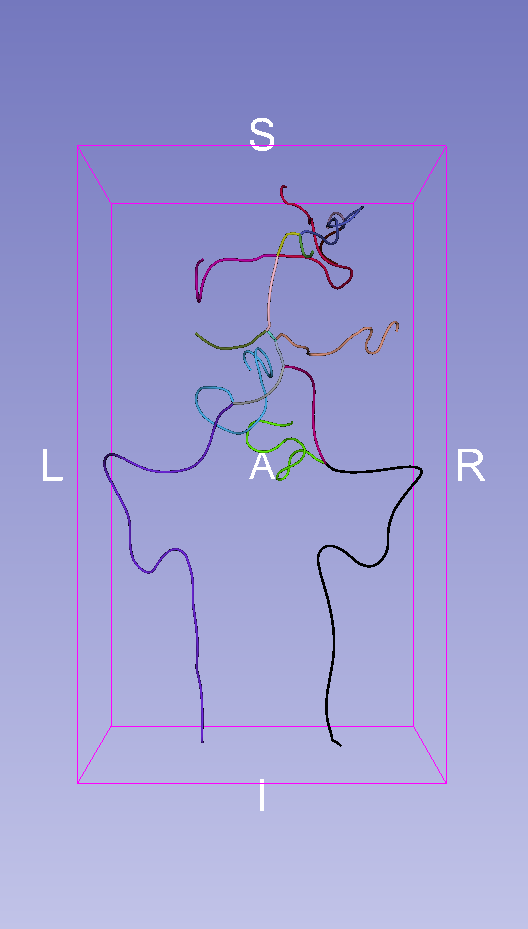
\includegraphics[width=\linewidth]{images/0053_extract3.png}
		\end{minipage}}
			\begin{minipage}{0.37\linewidth}
				{\small \begin{enumerate}
				\item<1-> load meshdata from \emph{vascularmodel.com} in Slicer 3D
				\item<2-> use VMTK plugin to determine start/end points
				\item<3-> extract 1D geometry
				\item<4-> save extracted geometry in table
		\end{enumerate}}
			\end{minipage}
	\end{minipage}
		\begin{minipage}{\linewidth}
			\begin{minipage}{0.075\linewidth}
				{\ }
			\end{minipage}
			\onslide<2->{\begin{minipage}{0.1\linewidth}
				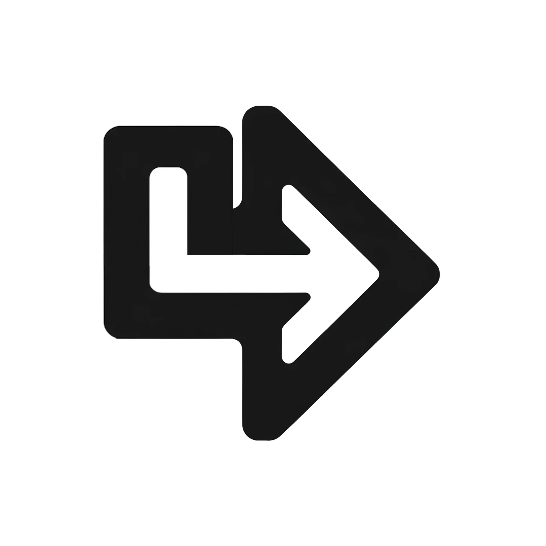
\includegraphics[width=\linewidth]{images/left_turn_arrow.eps}
			\end{minipage}
			\begin{minipage}{0.25\linewidth}
				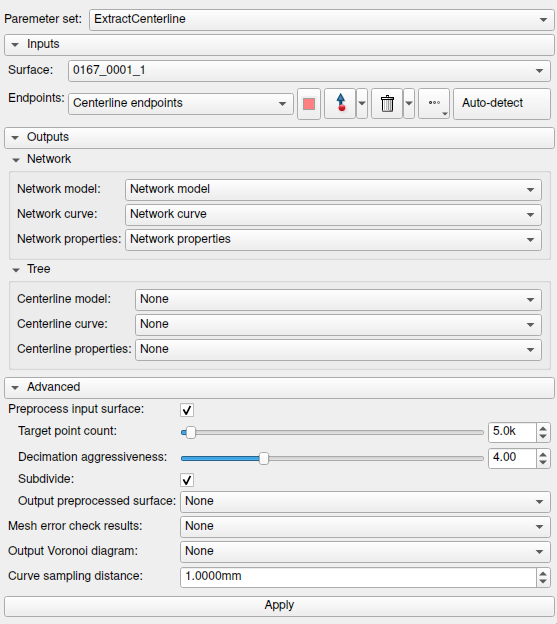
\includegraphics[width=\linewidth]{images/0053_extract2.png}
		\end{minipage}}
			\onslide<4->{\begin{minipage}{0.1\linewidth}
				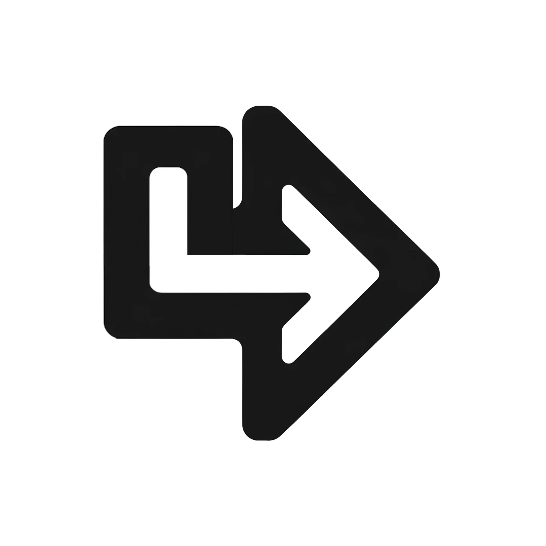
\includegraphics[width=\linewidth]{images/left_turn_arrow.eps}
		\end{minipage}
			\begin{minipage}{0.25\linewidth}
				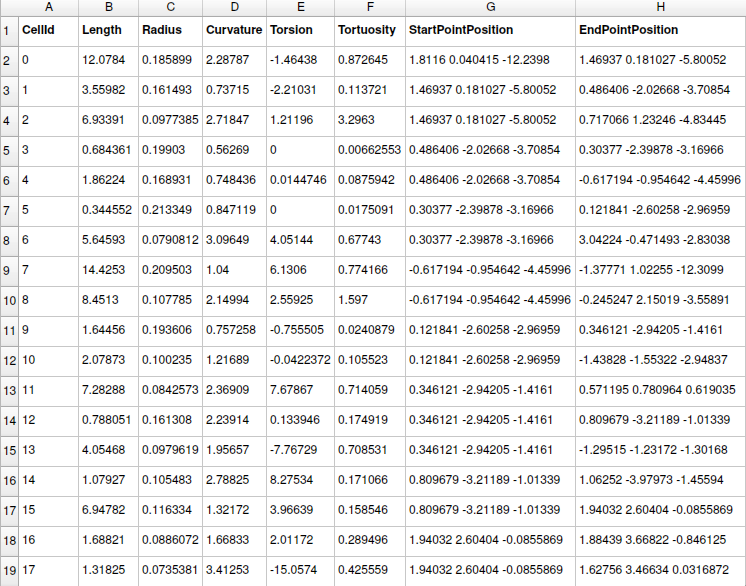
\includegraphics[width=\linewidth]{images/0053_extract4.png}
		\end{minipage}}
			\begin{minipage}{0.195\linewidth}
		\end{minipage}
		\end{minipage}
\end{frame}

%\begin{frame}
%	\frametitle{1D Geometry Extraction: Slicer 3D + VMTK}
%	\begin{center}
%		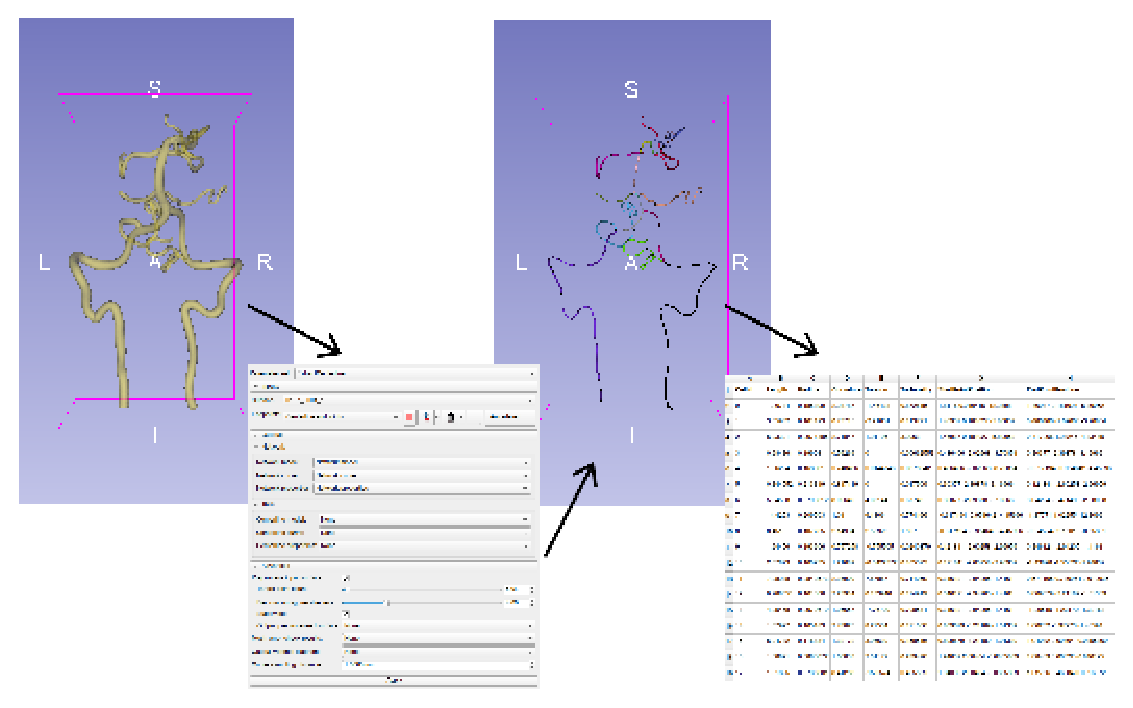
\includegraphics[width=\textwidth]{images/0053_extract.eps}
%	\end{center}
%\end{frame}

\againframe<4>{mp}

\begin{frame}
	\frametitle{Example: Bifurcation}
	\begin{figure}
		\begin{center}
			\begin{minipage}[t][0.35\paperheight][t]{\textwidth}
				\begin{minipage}{0.44\textwidth}
					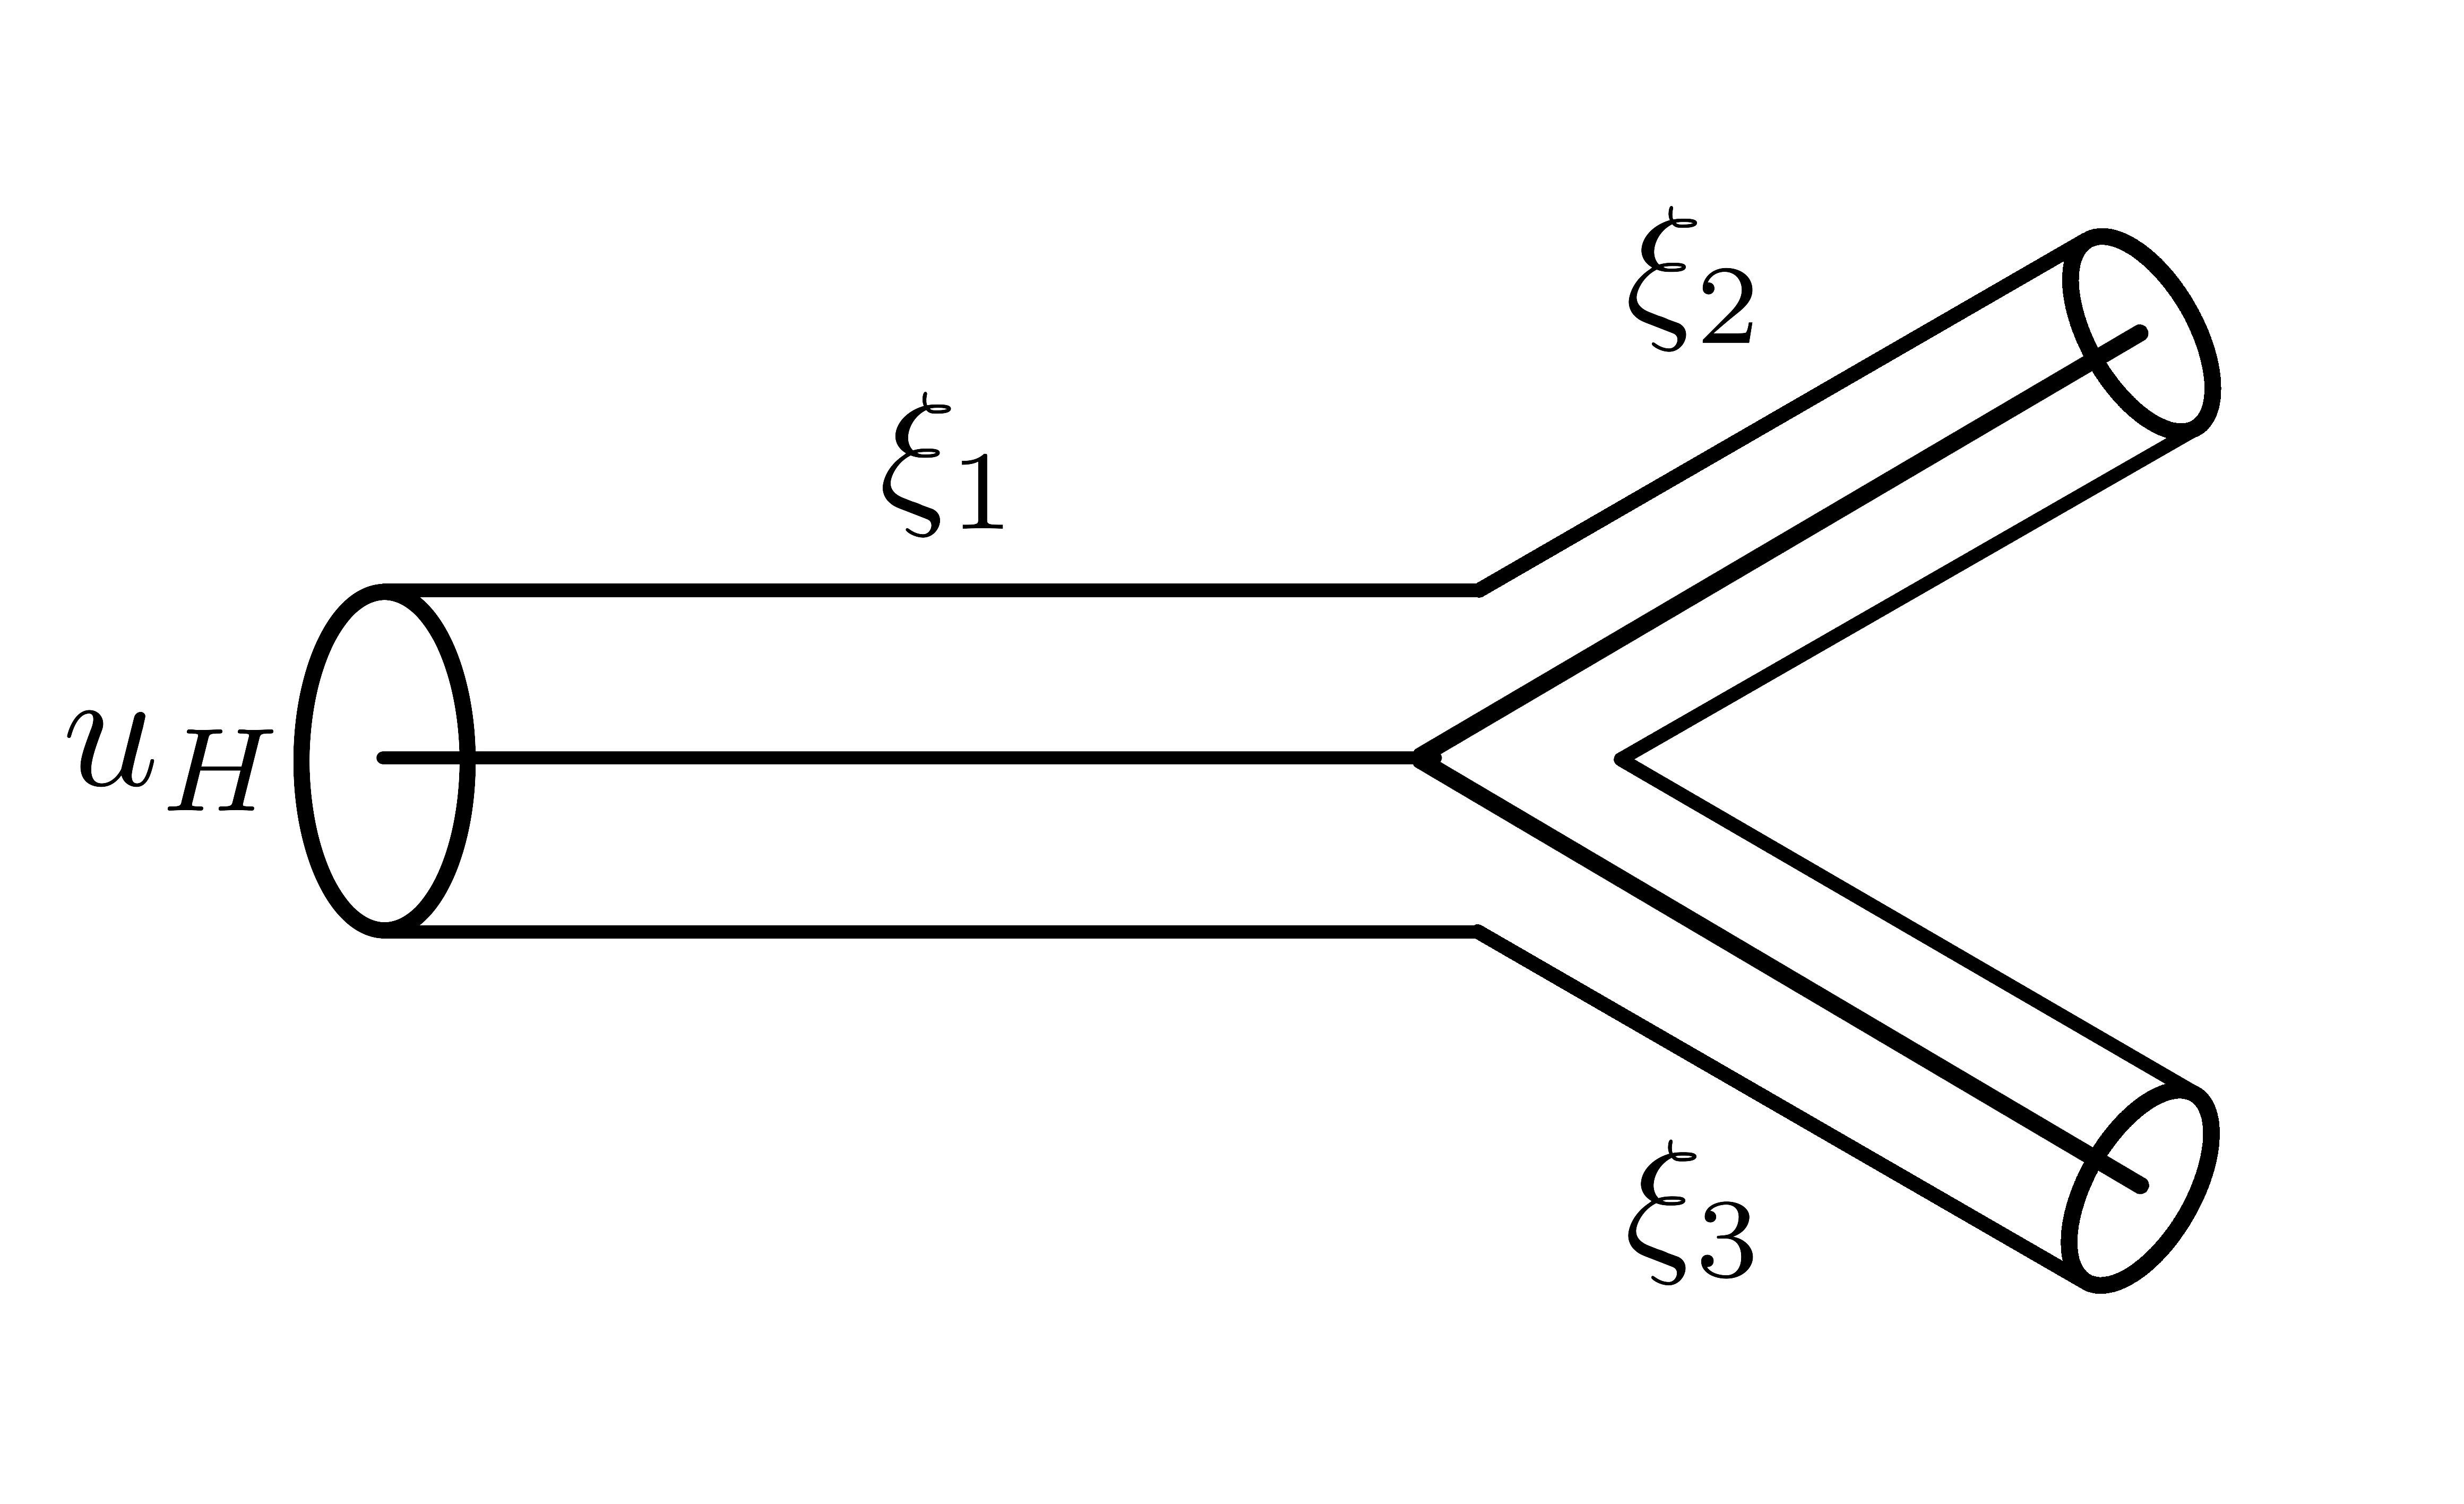
\includegraphics[width=\textwidth]{images/bifurcation.eps}
				\end{minipage}
				\hfill
				\begin{minipage}{0.09\textwidth}
					
\includegraphics[width=\textwidth]{images/right_arrow.png}
				\end{minipage}
				\hfill
				\begin{minipage}{0.44\textwidth}
					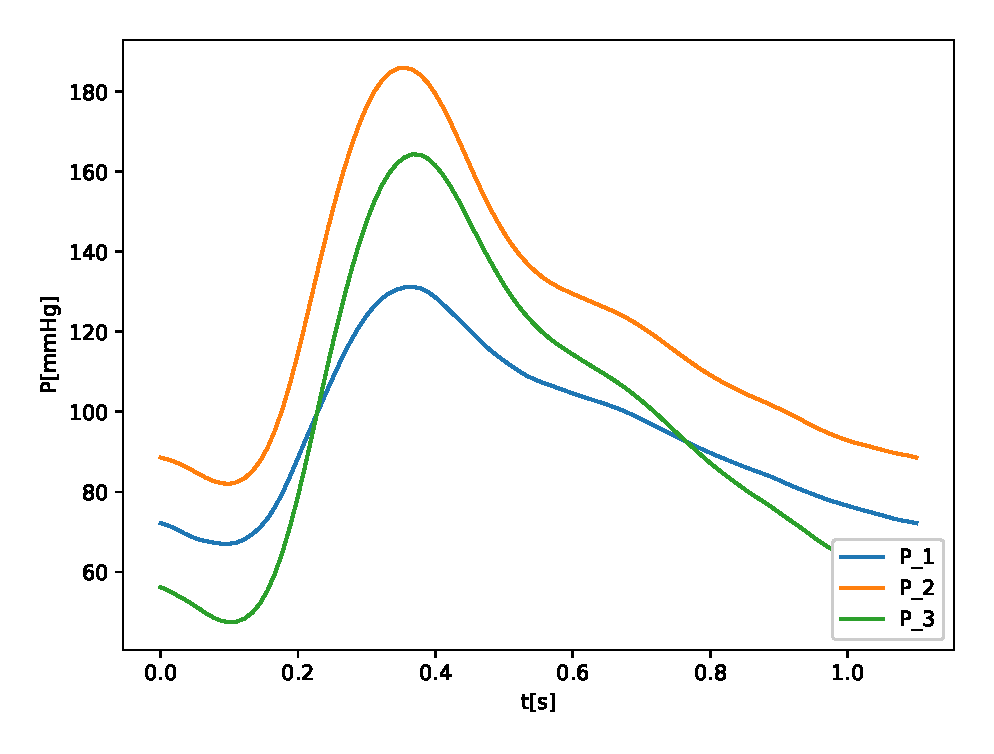
\includegraphics[width=\textwidth]{images/compare_output_params_P_P.eps}
				\end{minipage}
			\end{minipage}
		\end{center}
	\end{figure}
	\begin{minipage}[t][0.44\paperheight][t]{\textwidth}
	\end{minipage}
\end{frame}

\begin{frame}
	\frametitle{Example: Bifurcation}
	\begin{figure}
		\begin{center}
			\begin{minipage}[t][0.35\paperheight][t]{\textwidth}
				\begin{minipage}{0.44\textwidth}
					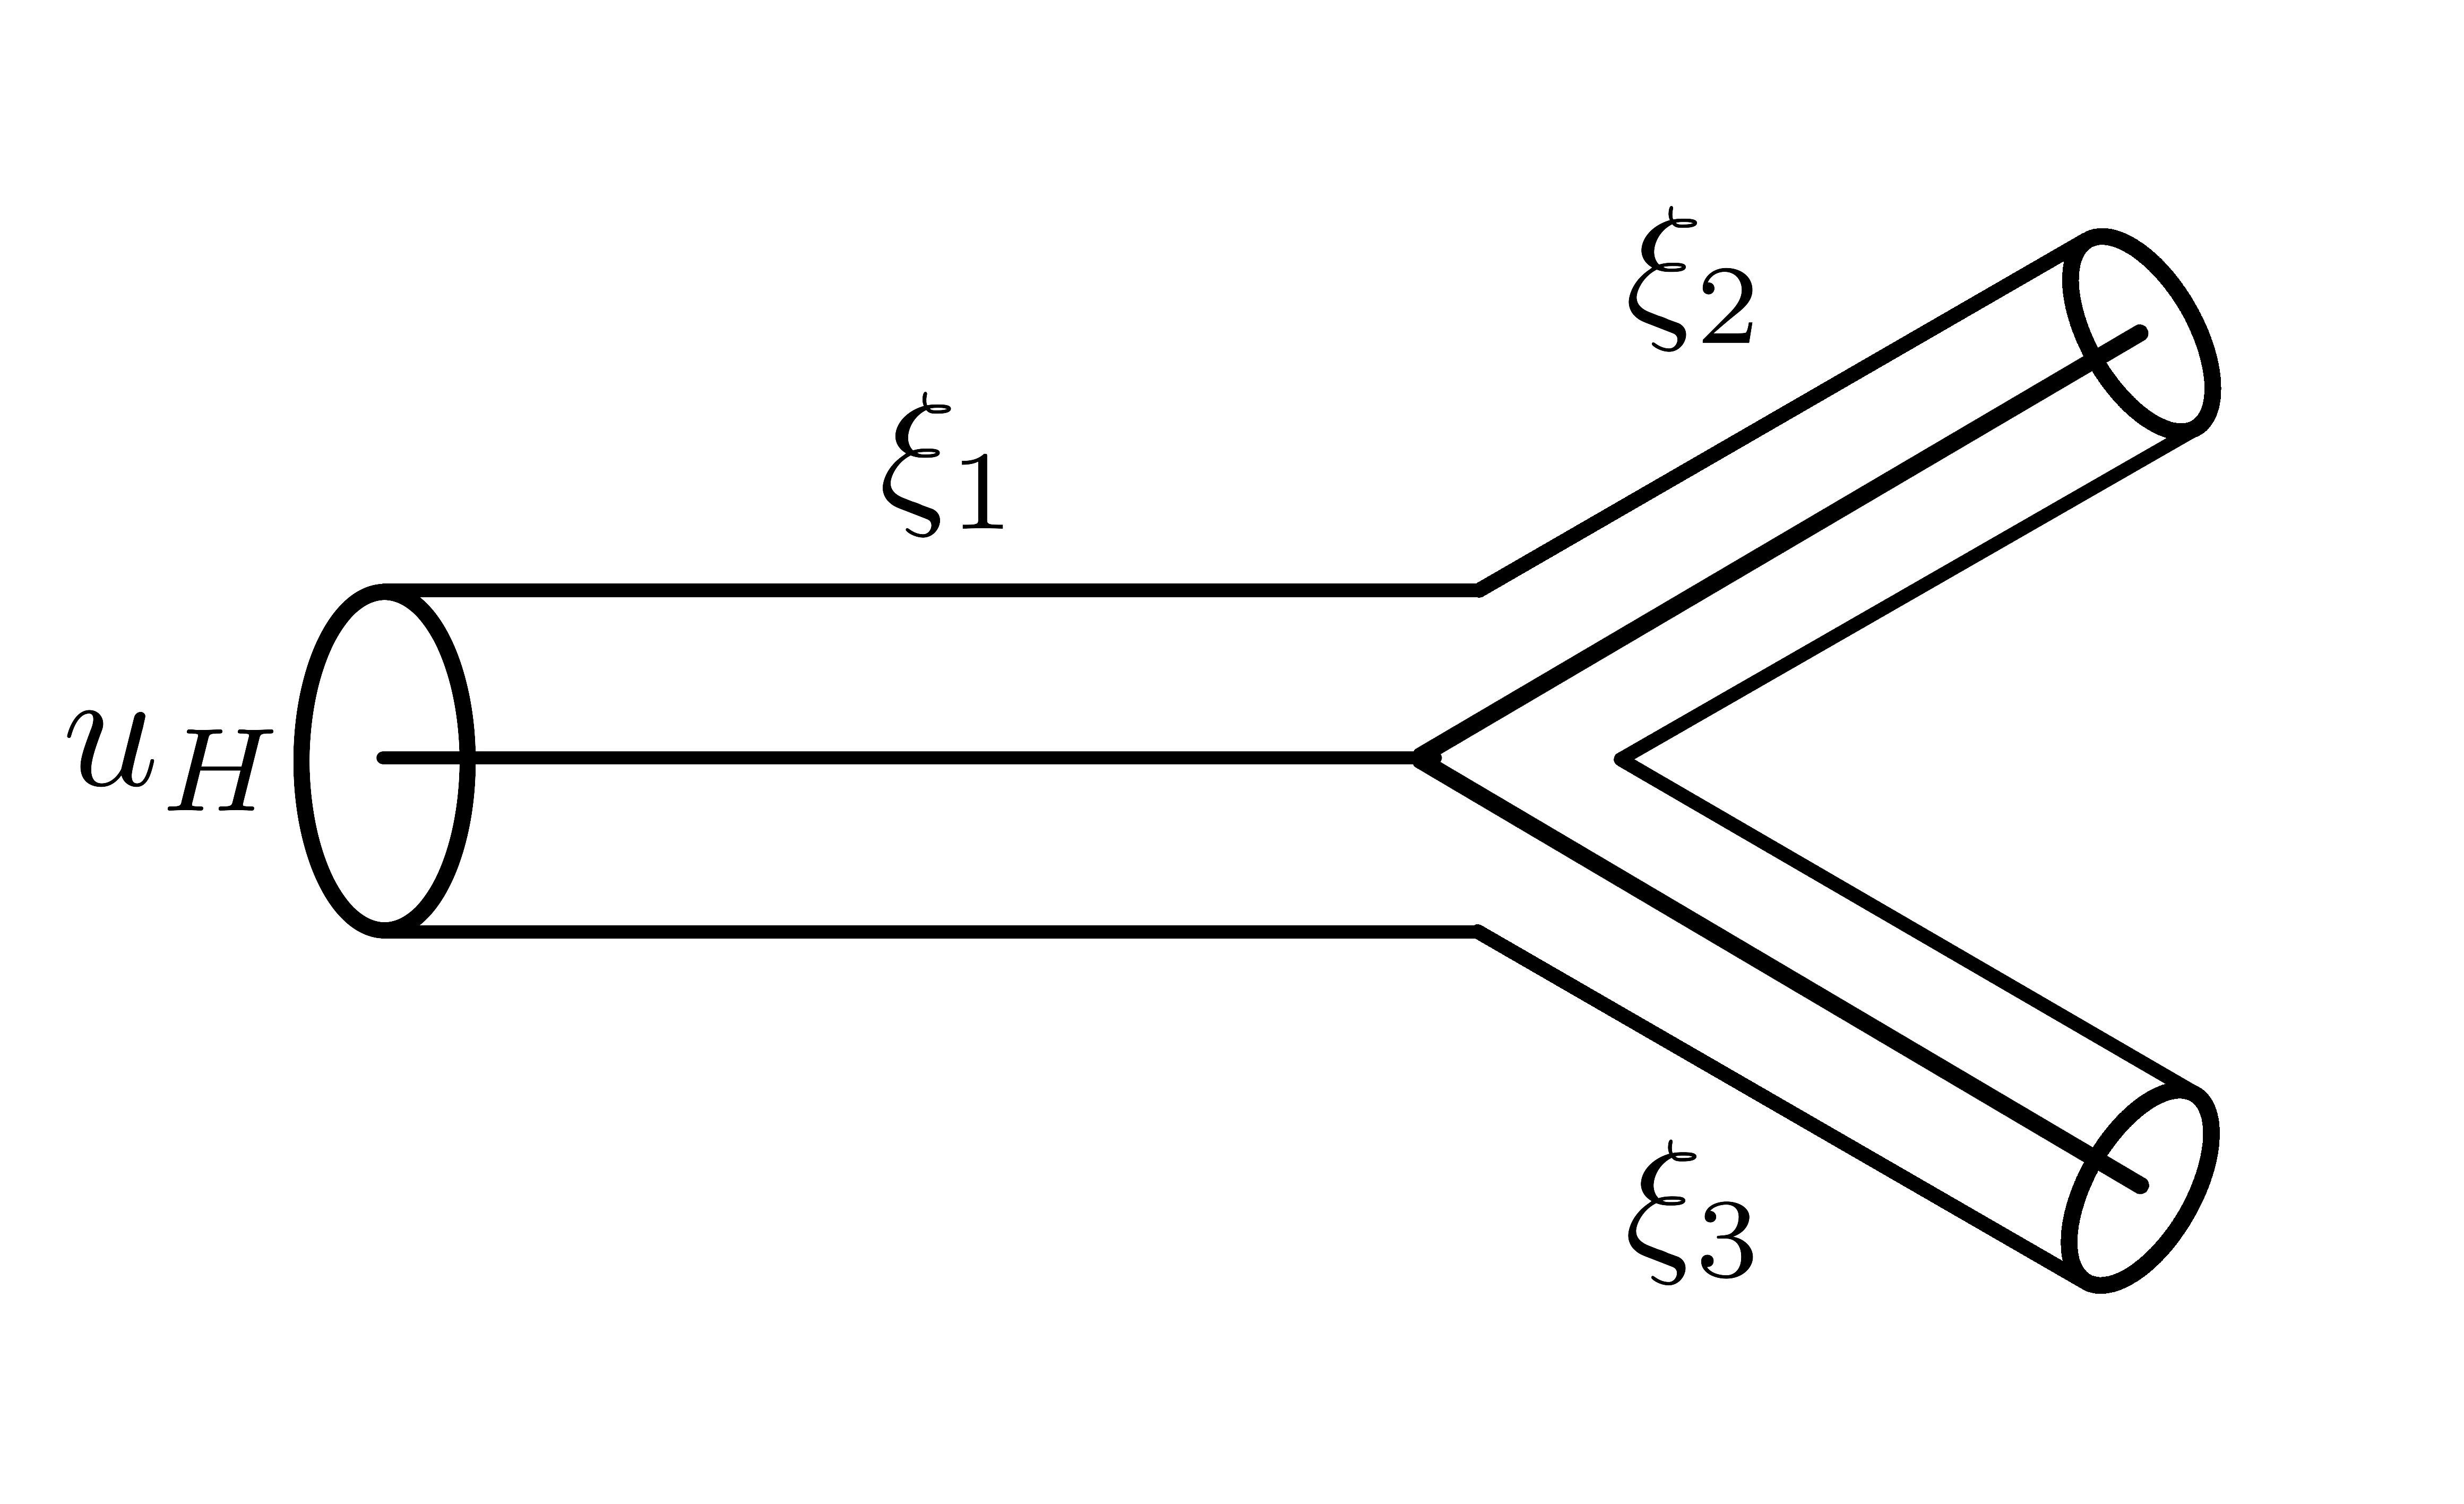
\includegraphics[width=\textwidth]{images/bifurcation.eps}
				\end{minipage}
				\hfill
				\begin{minipage}{0.09\textwidth}
					
\includegraphics[width=\textwidth]{images/right_arrow.png}
				\end{minipage}
				\hfill
				\begin{minipage}{0.44\textwidth}
					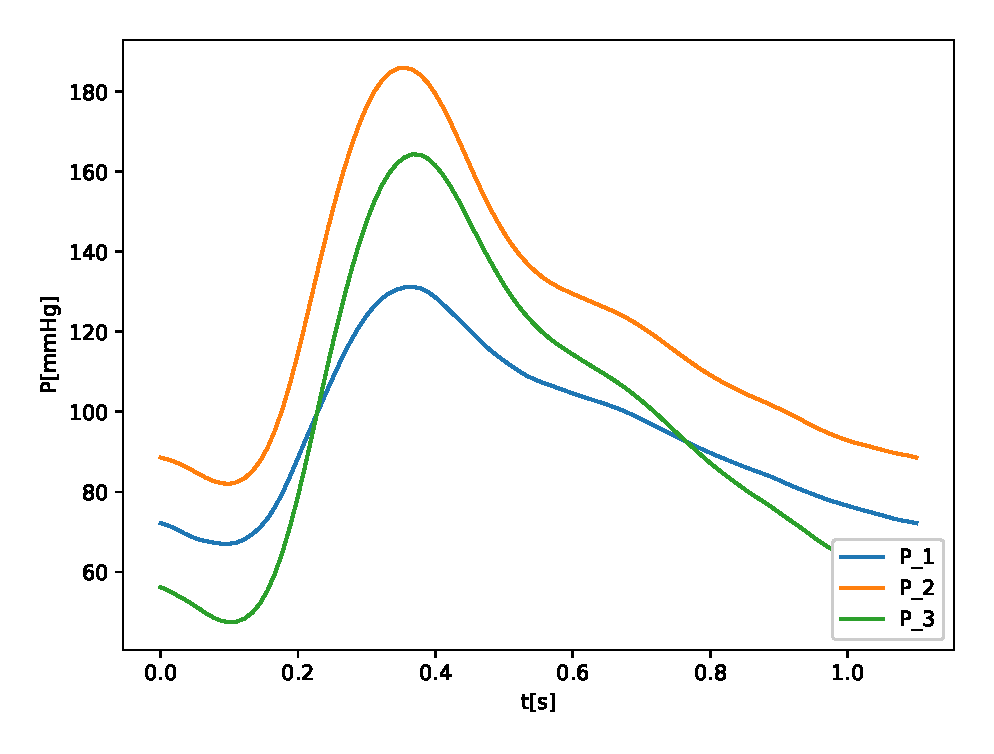
\includegraphics[width=\textwidth]{images/compare_output_params_P_P.eps}
				\end{minipage}
			\end{minipage}
			\begin{minipage}[t][0.34\paperheight][t]{\textwidth}
				\begin{minipage}{0.44\textwidth}
					\caption*{The bifurcation $\xi := \{u_H, \xi_1, \xi_2, \xi_3\}$ consists of a driving flow $u_H$ and three vessels: $\xi_1 := \{l^1, h_0^1, A_0^1, E^1\}$, $\xi_2 := \{l^2, h_0^2, A_0^2, E^2, R_1^2, C^2, R_2^2\}$, $\xi_3 := \{l^3, h_0^3, A_0^3, E^3, R_1^3, C^3, R_2^3\}.$}
				\end{minipage}
				\hfill
				\begin{minipage}{0.44\textwidth}
				\end{minipage}
			\end{minipage}
		\end{center}
	\end{figure}
	\begin{minipage}[t][0.1\paperheight][t]{\textwidth}
		{\tiny \centering 
			$u_H \hat{=}$ flow from heart,

			$l \hat{=}$ vessel length,
			$h_0 \hat{=}$ reference vessel wall thickness,
			$A_0 \hat{=}$ reference cross-section,

			$E \hat{=}$ Young's modulus,
			$R_1, C, R_2 \hat{=}$ Windkessel parameters.
		\par}
	\end{minipage}
\end{frame}
\begin{frame}
	\frametitle{Example: Bifurcation}
	\begin{figure}
		\begin{center}
			\begin{minipage}[t][0.35\paperheight][t]{\textwidth}
				\begin{minipage}{0.44\textwidth}
					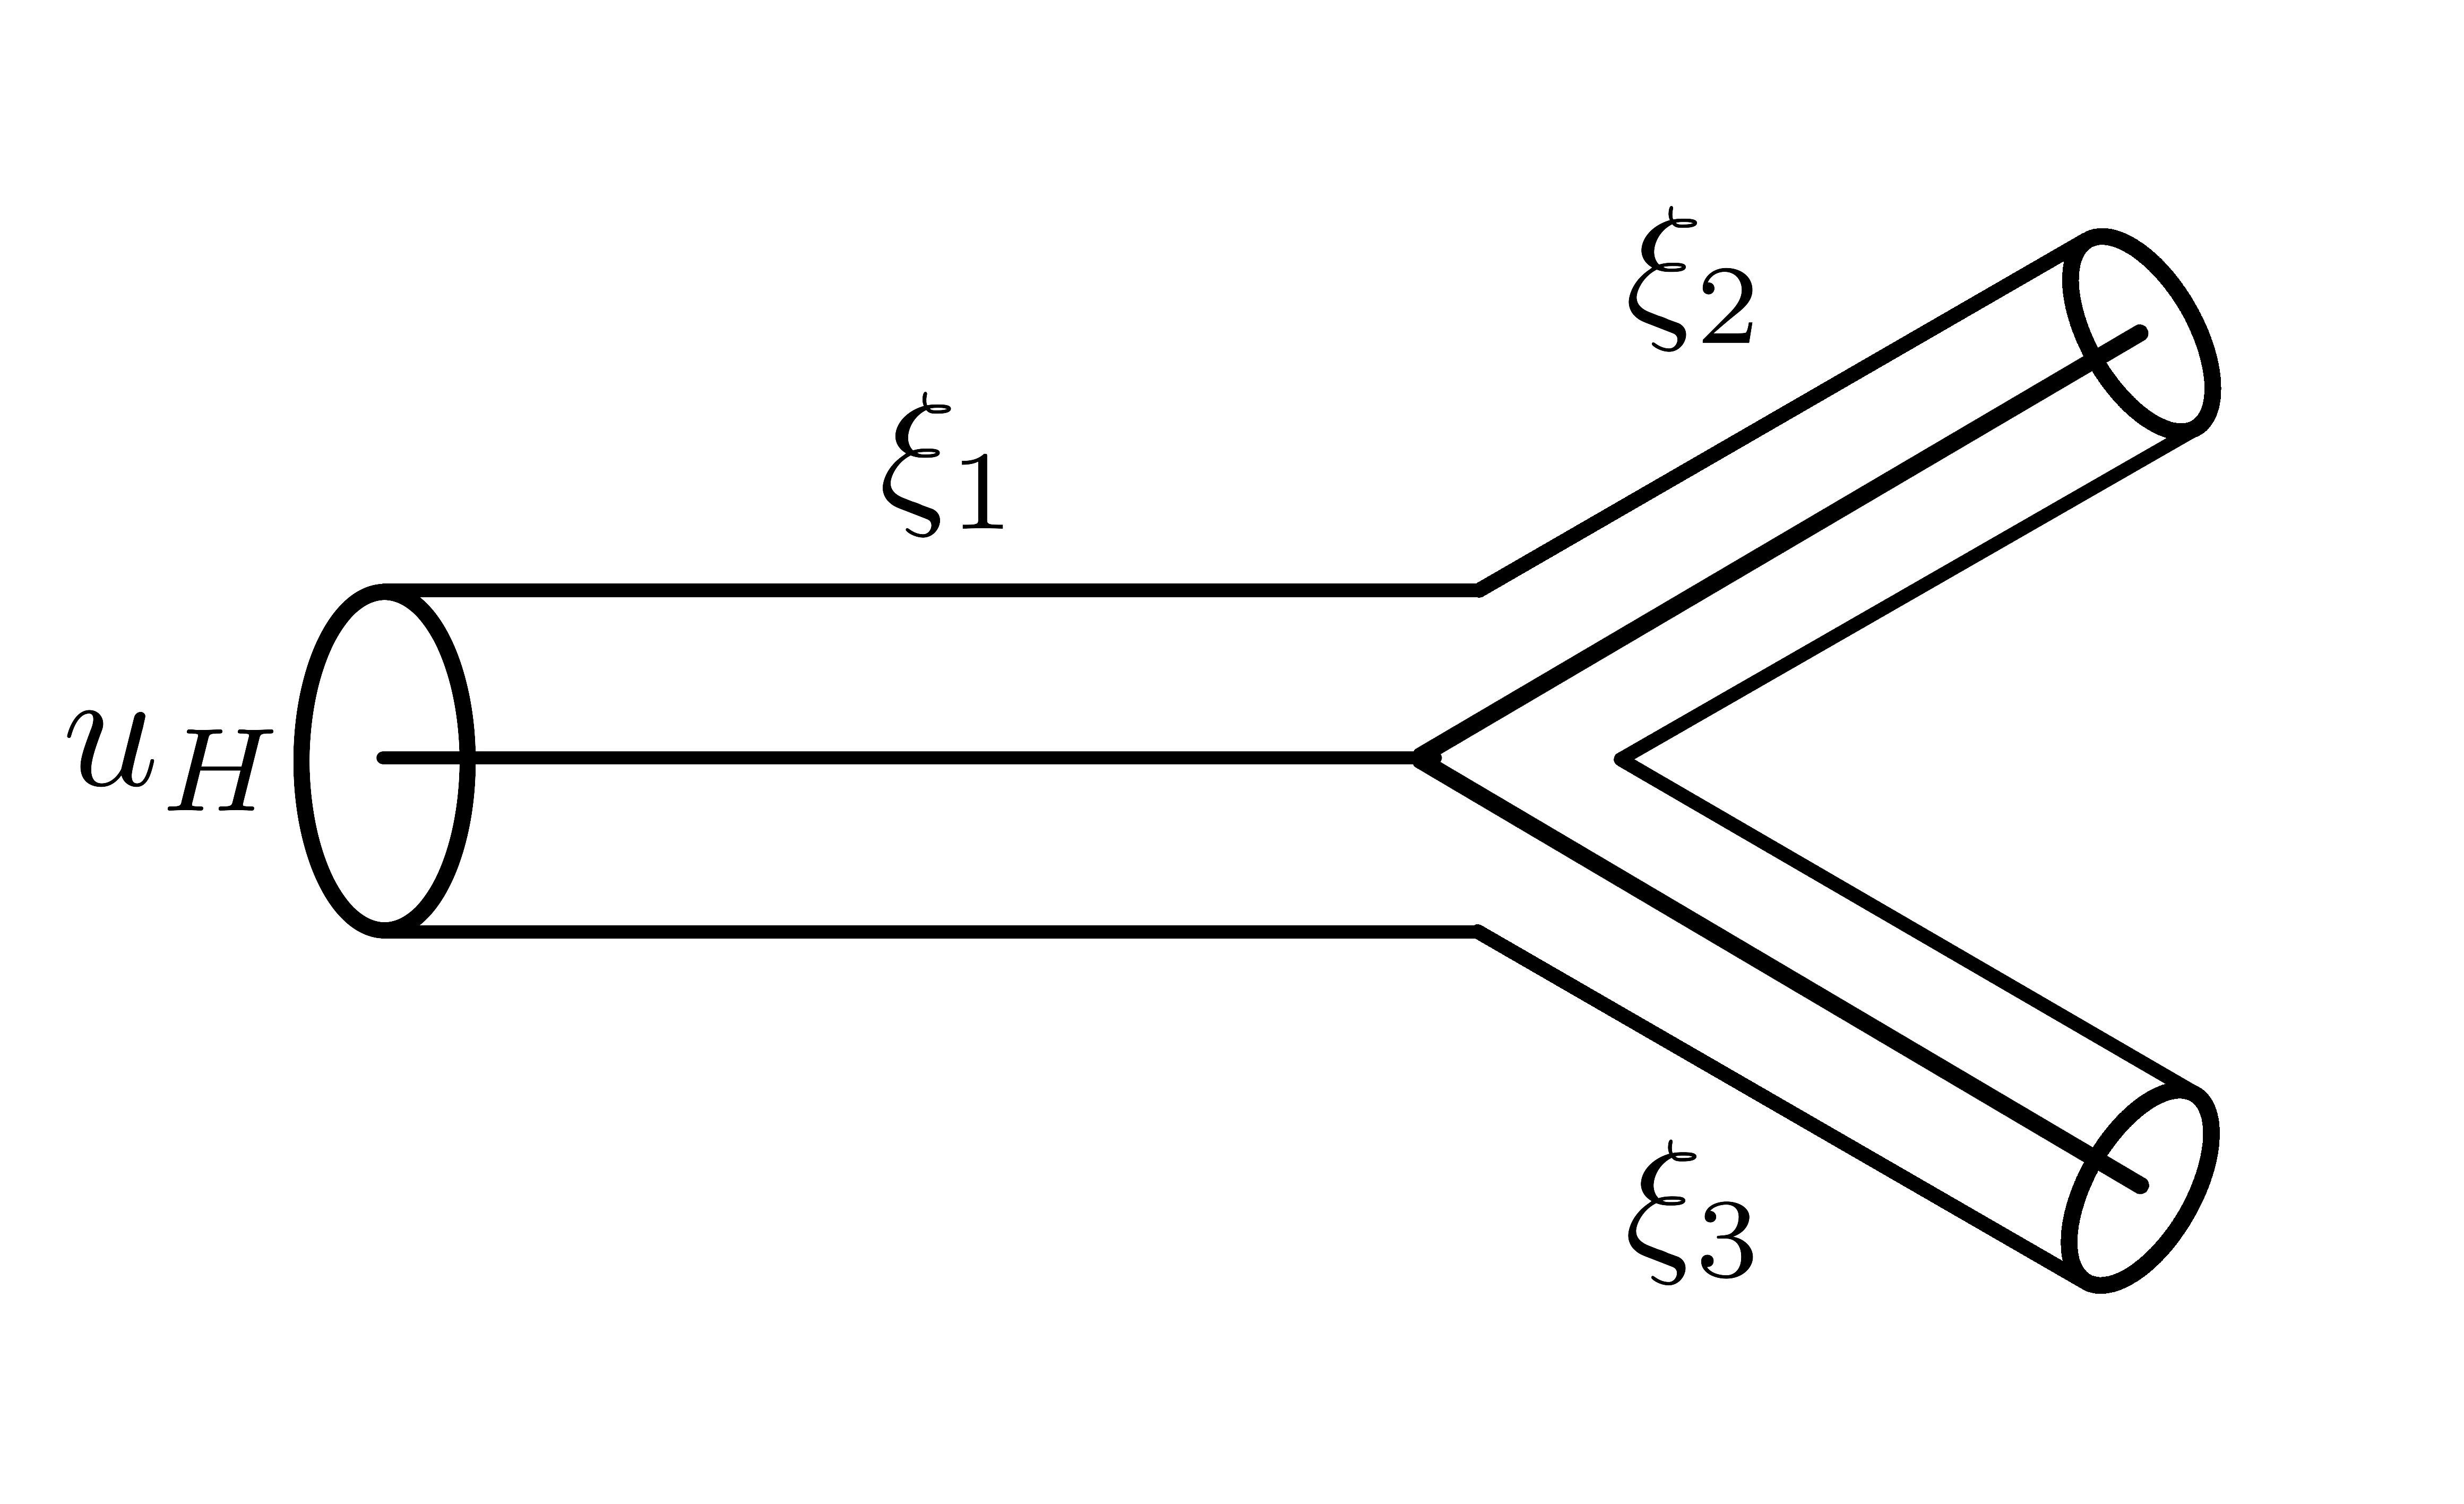
\includegraphics[width=\textwidth]{images/bifurcation.eps}
				\end{minipage}
				\hfill
				\begin{minipage}{0.09\textwidth}
					
\includegraphics[width=\textwidth]{images/right_arrow.png}
				\end{minipage}
				\hfill
				\begin{minipage}{0.44\textwidth}
					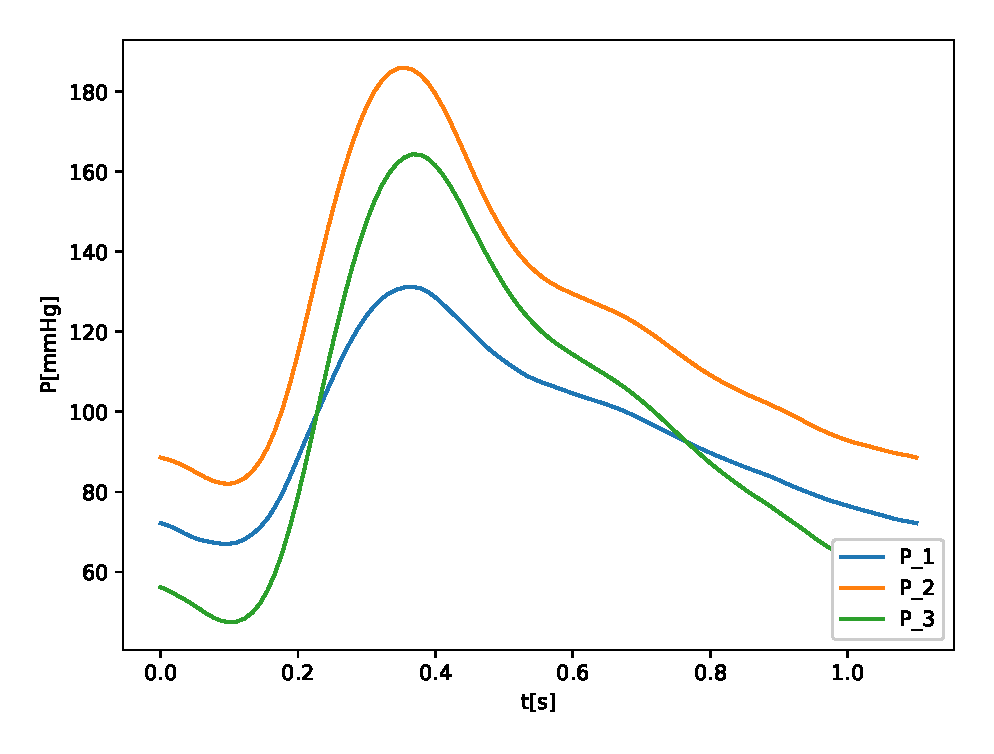
\includegraphics[width=\textwidth]{images/compare_output_params_P_P.eps}
				\end{minipage}

				%\begin{minipage}{0.48\textwidth}
				%	\captionof{figure}{test}
				%\end{minipage}
				%\hfill
				%\begin{minipage}{0.48\textwidth}
				%	\captionof{figure}{test}
				%\end{minipage}
			\end{minipage}
			\hfill
			\begin{minipage}[t][0.34\paperheight][t]{\textwidth}
				\begin{minipage}{0.44\textwidth}
					\caption*{The bifurcation $\xi := \{u_H, \xi_1, \xi_2, \xi_3\}$ consists of a driving flow $u_H$ and three vessels: $\xi_1 := \{l^1, h_0^1, A_0^1, E^1\}$, $\xi_2 := \{l^2, h_0^2, A_0^2, E^2, R_1^2, C^2, R_2^2\}$, $\xi_3 := \{l^3, h_0^3, A_0^3, E^3, R_1^3, C^3, R_2^3\}.$}
				\end{minipage}
				\hfill
				\begin{minipage}{0.44\textwidth}
					\caption*{Altering the Windkessel parameters $(R_1,C,R_2)$ leads to vastly different pressure waves being simulated.}
					\vfill
				\end{minipage}
			\end{minipage}
		\end{center}
	\end{figure}
	\hfill
	\begin{minipage}[t][0.1\paperheight][t]{\textwidth}
		{\tiny \centering 
			$u_H \hat{=}$ flow from heart,

			$l \hat{=}$ vessel length,
			$h_0 \hat{=}$ reference vessel wall thickness,
			$A_0 \hat{=}$ reference cross-section,

			$E \hat{=}$ Young's modulus,
			$R_1, C, R_2 \hat{=}$ Windkessel parameters.
		\par}
	\end{minipage}
\end{frame}

\begin{frame}
	\frametitle{Example: Bifurcation}
	\begin{figure}
		\begin{center}
			\begin{minipage}[t][0.35\paperheight][t]{\textwidth}
				\begin{minipage}{0.44\textwidth}
					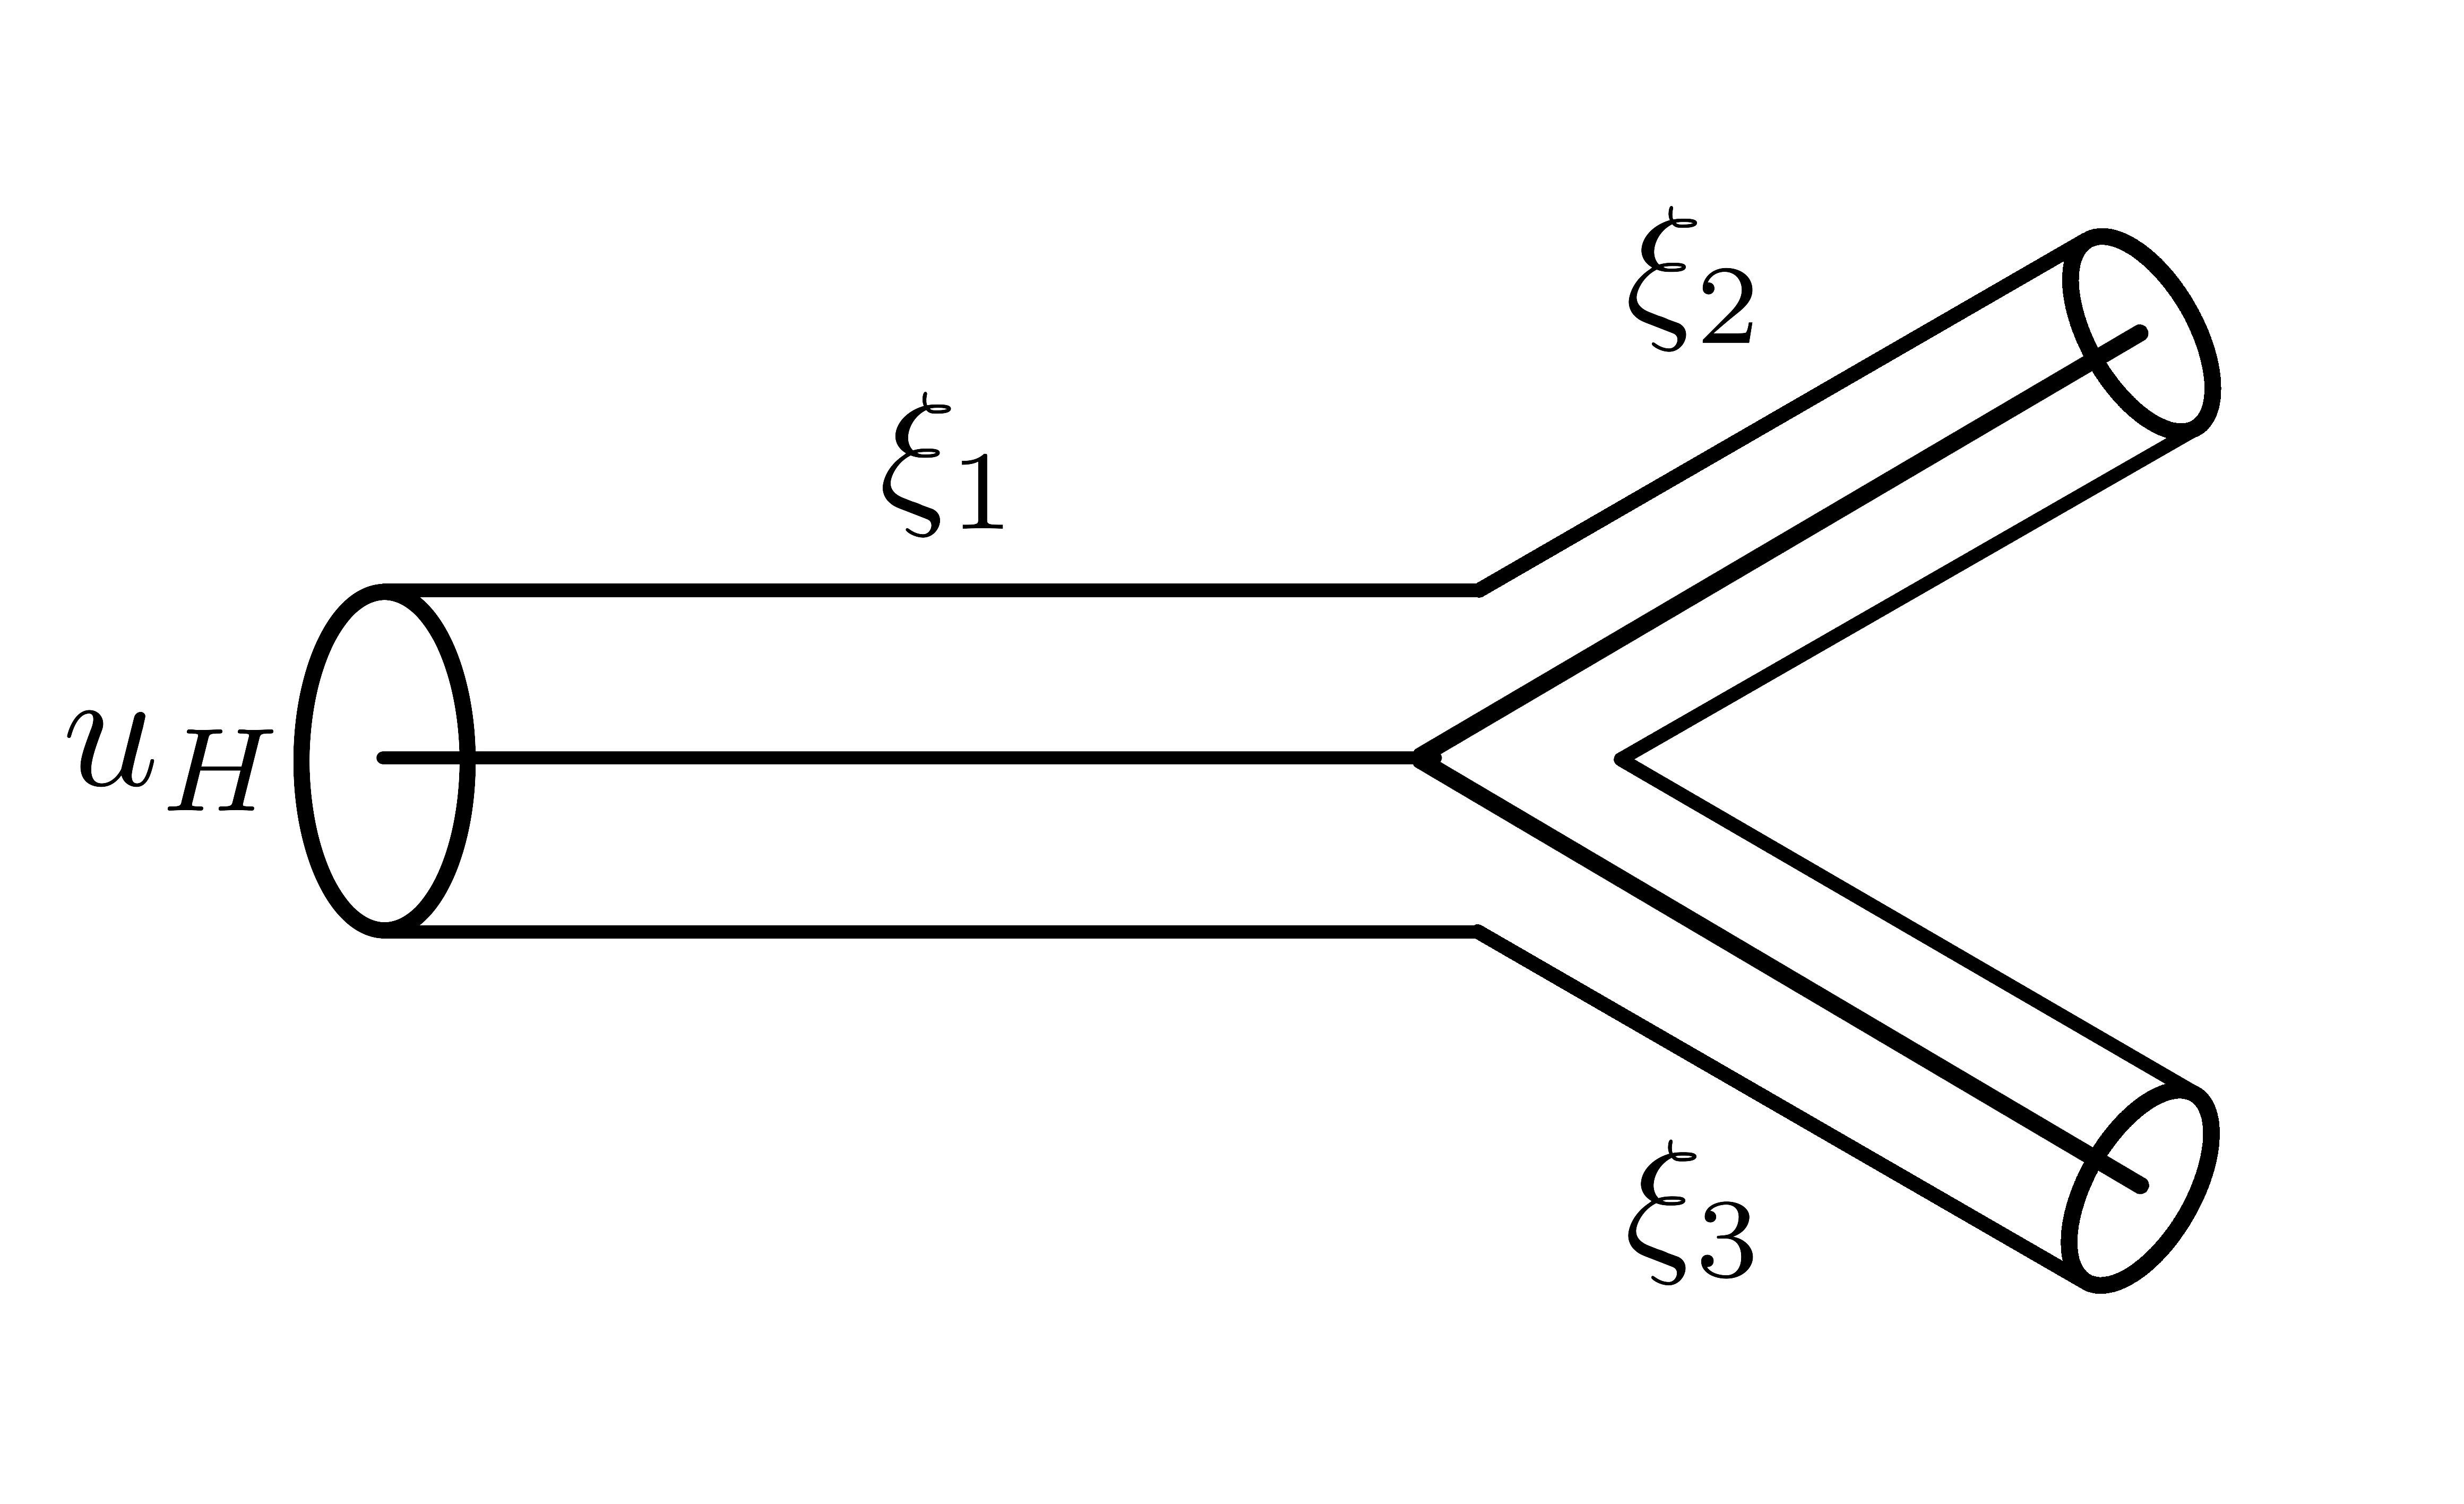
\includegraphics[width=\textwidth]{images/bifurcation.eps}
				\end{minipage}
				\hfill
				\begin{minipage}{0.09\textwidth}
					
\includegraphics[width=\textwidth]{images/right_arrow.png}
				\end{minipage}
				\hfill
				\begin{minipage}{0.44\textwidth}
					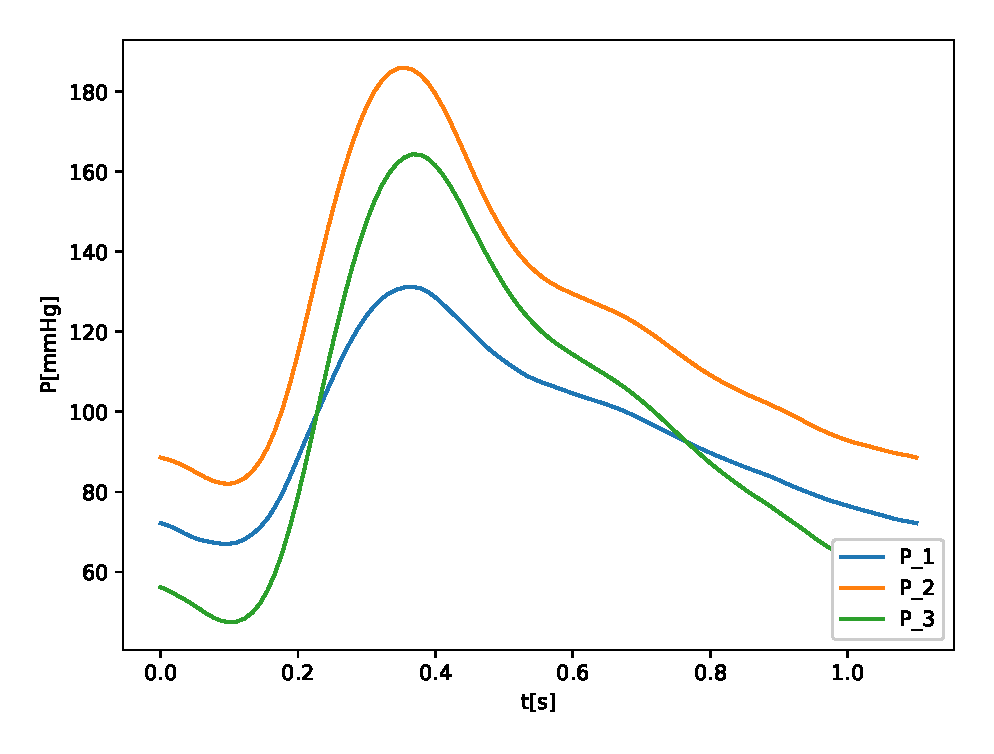
\includegraphics[width=\textwidth]{images/compare_output_params_P_P.eps}
				\end{minipage}
			\end{minipage}
		\end{center}
	\end{figure}
	\begin{minipage}[t][0.44\paperheight][t]{\textwidth}
		\hfill
		\begin{block}{Conclusion}
			The parameters are patient dependent and can heavily influence the simulation outcome. Therefore efficient methods of determining these parameters (solving the inverse problem) are necessary.
		\end{block}
	\end{minipage}
\end{frame}

\begin{frame}
	\frametitle{Setting Parameters: Python Script}
	\onslide<1->{\begin{minipage}{0.25\textwidth}
		\begin{figure}
			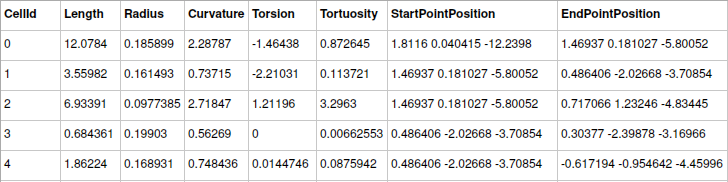
\includegraphics[width=\textwidth]{images/0053_extract4_cropped.png}
			\caption*{dimensions and connectivity}
			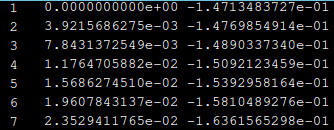
\includegraphics[width=\textwidth]{images/config0.png}
			\caption*{inflow data}
			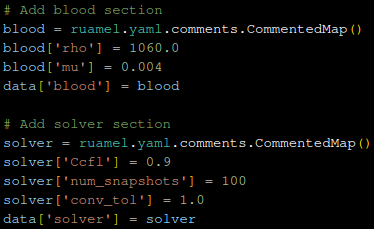
\includegraphics[width=\textwidth]{images/config1.png}
			\caption*{simulation constants}
		\end{figure}
\end{minipage}}
	\onslide<2->{\begin{minipage}{0.1\textwidth}
		
\includegraphics[width=\textwidth]{images/right_arrow.png}
	\end{minipage}
	\begin{minipage}{0.25\textwidth}
		\begin{figure}
			\resizebox{\linewidth}{!}{\begin{minipage}{2.3\textwidth}
					\begin{align*}
						P_{mean} &:= \frac{120 \text{mmHg}}{80 \frac{\text{ml}}{\text{s}}}, \  Q_{car} := 80 \frac{\text{ml}}{\text{s}}, \\
						R_{tot} &:= \frac{P_{mean}}{Q_{car}}, \ C_{tot} := 10^{-3} \frac{\text{cm}^5}{\text{dyne}}, \\
						\xi_i &:= \frac{\sum_{j \in I} A_{0,j}}{A_{0,i}}, \\
						R_{tot,i} &:= \xi_i R_{tot}, \ C_{tot,i} := \frac{1}{\xi_i} C_{tot}, \\
						R_{1,i} &:= \frac{9}{100} R_{tot,i}, \ R_{2,i} := \frac{91}{100} R_{tot,i}.
					\end{align*}
			\end{minipage}}
			\caption*{Windkessel parameters}
			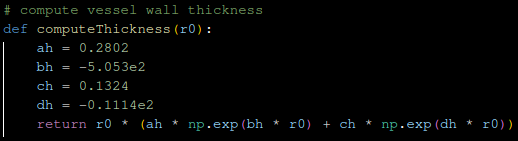
\includegraphics[width=\textwidth]{images/config2.png}
			\caption*{vessel wall thickness}
			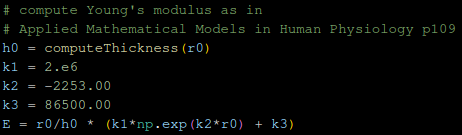
\includegraphics[width=\textwidth]{images/config3.png}
			\caption*{Young's modulus}
		\end{figure}
\end{minipage}}
	\onslide<3->{\begin{minipage}{0.1\textwidth}
		
\includegraphics[width=\textwidth]{images/right_arrow.png}
	\end{minipage}
	\begin{minipage}{0.25\textwidth}
		\begin{figure}
			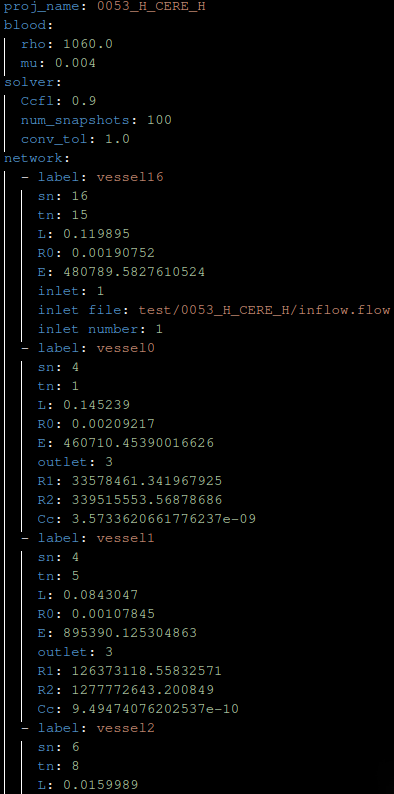
\includegraphics[width=\textwidth]{images/config4.png}
			\caption*{YML configuration}
		\end{figure}

\end{minipage}}
\end{frame}

%\begin{frame}
%	\frametitle{Solving the Inverse Problem}
%\begin{minipage}[t][0.35\paperheight][t]{\textwidth}
%\begin{tabular}{| m{2cm} | m{2cm}| m{2cm} | m{2.4cm} | } 
%	\hline
%	approach & method & speed & interpretability\\ 
%	\hline
%	\hline
%	"classical" numerical methods & stochastic & slower & high \\ 
%	\hline
%	deep learning & gradient based & faster & low \\ 
%	\hline
%\end{tabular}
%\end{minipage}
%\hfill
%\begin{minipage}[t][0.35\paperheight][t]{\textwidth}
%\end{minipage}
%\end{frame}
%
%\begin{frame}
%	\frametitle{Solving the Inverse Problem}
%\begin{minipage}[t][0.35\paperheight][t]{\textwidth}
%\begin{tabular}{| m{2cm} | m{2cm}| m{2cm} | m{2.4cm} | } 
%	\hline
%	approach & method & speed & interpretability\\ 
%	\hline
%	\hline
%	"classical" numerical methods & stochastic & slower & high \\ 
%	\hline
%	deep learning & gradient based & faster & low \\ 
%	\hline
%\end{tabular}
%\end{minipage}
%\hfill
%\begin{minipage}[t][0.35\paperheight][t]{\textwidth}
%	\begin{block}{Conclusion}
%		When solving the inverse problem "classical" numerical methods are inefficient due to not having gradients available while deep learning approaches lack interpretability.
%		A numerical solver that provides gradient information w.r.t. it's parameters would provide a fast a interpretable way of solving the inverse problem.
%	\end{block}
%\end{minipage}
%
%\end{frame}

%\begin{frame}
%	\frametitle{Introduction}
%	\begin{block}{What is jaxFlowSim?}
%		\begin{itemize}
%			\item 1D-haemodynamics solver
%			\item written in JAX
%			\item differentiable
%		\end{itemize}
%	\end{block}
%	\vspace{5mm}
%\end{frame}

%\begin{frame}
%	\frametitle{Motivation}
%	\begin{block}{Use and Novelty}
%		\begin{itemize}
%			\item towards personalised medicine
%			\item parameter inference
%			\item sensitivity analysis
%		\end{itemize}
%	\end{block}
%	\vspace{5mm}
%\end{frame}

\againframe<5>{mp}

\begin{frame}<1>[label=nse]
	\frametitle{1D-Navier Stokes Equations}
	\begin{equation}
		\begin{aligned}
			\frac{\partial \mathbf{U}}{\partial t} + \frac{\partial \mathbf{F} \left(
			\mathbf{U} \right)}{\partial z} &= \mathbf{S} \left( \mathbf{U} \right), \ t>0, \
			z \in \left[ 0,l \right], \only<1>{\\
			\mathbf{U} \left( z;0 \right) &= \mathbf{U}_0 \left( z \right), \ z \in \left[ 0,l \right], \\
			\mathbf{U} \left( 0;t \right) &= \mathbf{U}_L \left( t \right), \ t>0,\\
		\mathbf{U} \left( l;t \right) &= \mathbf{U}_R \left( t \right), \ t>0,}
		\end{aligned} \label{eq:1deqs3}
	\end{equation}
	\begin{equation}
		\mathbf{U} :=
		\begin{bmatrix}
			A \\
			Q
		\end{bmatrix}, \ 
		\mathbf{F} \left( \mathbf{U} \right) :=
		\begin{bmatrix}
			Q \\
			\frac{Q^2}{A} + \frac{\beta A^{\frac{3}{2}}}{3\rho\sqrt{A_0}}
		\end{bmatrix}, \ 
		\mathbf{S} \left( \mathbf{U} \right) :=
		\begin{bmatrix}
			0 \\
			-22\frac{\mu}{\rho}\frac{Q}{A}
		\end{bmatrix}.
	\end{equation}

	\vfill

	{\tiny \centering 
		\only<1>{$\mathbf{U_0} \hat{=}$ initial condition, 
		$\mathbf{U_L} \hat{=}$ left boundary values,
	$\mathbf{U_R} \hat{=}$ right boundary values,}

		$l \hat{=}$ vessel length,
		$A \hat{=}$ cross-section,
		$A_0 \hat{=}$ reference cross-section,
		$Q \hat{=}$ volumetric flow-rate,

		$\beta \hat{=}$ elasticity coefficient,
		$\rho \hat{=}$ blood density,
		$\mu \hat{=}$ blood dynamic viscosity. 
	\par}

	\only<2->{\vfill

		\begin{block}{Conservative Form with Source Term}
		\begin{itemize}
			\onslide<3->{\item conservation of mass (continuity equation)}
			\onslide<4->{\item conservation of momentum}
			\onslide<5->{\item no energy equation (incompressible Newtonian fluid)}
		\end{itemize}
			
\end{block}}



\end{frame}

\againframe<2>{nse}
\againframe<3>{nse}
\againframe<4>{nse}
\againframe<5>{nse}

\begin{frame}<1>[label=tl]
	\frametitle{Tube Law}
	\begin{align}
		P(z;t) &:= P_{ext}(z;t) + \beta \left( \sqrt{\frac{A(z;t)}{A_0(z)}}-1 \right),      \label{eq:p_tot}\\
		\beta(z) &:=  \frac{\sqrt{\pi} E h_0(z)}{(1-\nu^2) \sqrt{A_0(z)}},\  z \in \left[ 0,l \right], \ t > 0. 
	\end{align}

	\vfill

	{\tiny \centering 
		$P \hat{=}$ pressure,
		$P_{ext} \hat{=}$ external pressure,

		$l \hat{=}$ vessel length,
		$A \hat{=}$ cross-section,
		$A_0 \hat{=}$ reference cross-section,

		$E \hat{=}$ Young's modulus,
		$h_0 \hat{=}$ reference vessel wall thickness,
		$\nu \hat{=}$ Poisson's ratio (elasticity parameter). 
	\par}
		\onslide<1->{\begin{block}{Fluid-Structure Interaction}
			\begin{itemize}
			\onslide<2->{\item $P(z;t)$ describes fluid structure interaction}
			\onslide<3->{\item $\beta(z)$ quantifies structure}
			\end{itemize}
	\end{block}}
\end{frame}

\againframe<2>{tl}
\againframe<3>{tl}

\begin{frame}<1>[label=ic]
	\frametitle{Initial Conditions (IC)}
		\onslide<1->{\begin{minipage}{0.37\textwidth}
			\begin{block}{Steady State}
				Since good IC are not known trivial ones are set and the simulation is run until a steady state is reached.
			\end{block}

	\end{minipage}}
		\hfill
		\onslide<3->{\begin{minipage}{0.57\textwidth}
			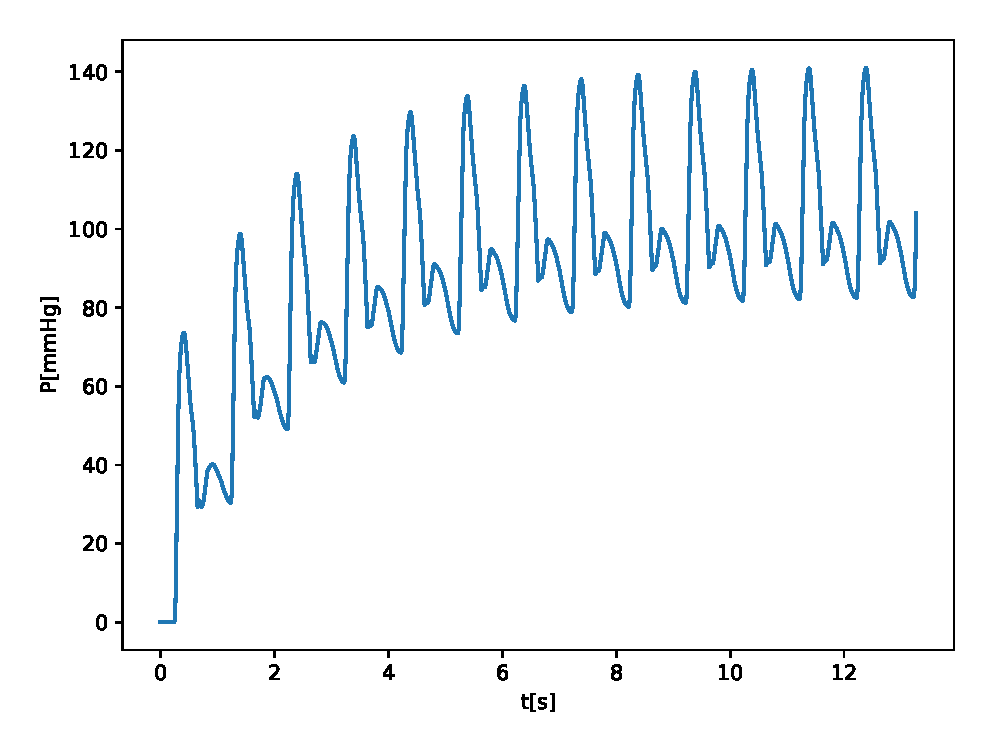
\includegraphics[width=\textwidth]{images/adan56_tibiofibular_trunk_L_P_steady_state.eps}
	\end{minipage}}
		\onslide<2->{\begin{align}
			u(z;0) &\equiv 0, &z \in [0,l],\\
			A(z;0) &= A_0(z), &z \in [0,l], \\
			Q(z;0) &= u(z;0)A(z;0) \equiv 0, &z \in [0,l].
	\end{align}}
\end{frame}

\againframe<2>{ic}
\againframe<3>{ic}

\begin{frame}
	\frametitle{Inlets, Junctions, Outlets}
	\begin{block}{Inlets}
		\onslide<2->{set $P$ or $Q$ from data}
	\end{block}
	\begin{block}{Junctions}
		\onslide<3->{solve linear system of equations consisting of:
		\begin{itemize}
			\item conservation of mass and
			\item conservation of momentum.
	\end{itemize}}
	\end{block}
	\begin{block}{Outlets}
		\onslide<4->{0D-/ lumped parameter model: three element Windkessel (RCR) model}
\end{block}
\end{frame}


%\begin{frame} [fragile]
%	\frametitle{Code Structure}
%	\begin{lstlisting}[basicstyle=\fontsize{7}{7}\selectfont\ttfamily, language=Python, caption={$dt \hat{=}$timestep(CFL), setBoundaryValues$\hat{=}$inlet(from data), outlet(Windkessel),junctions(conservation laws), muscl$\hat{=}$Monotonic Upstream-centered Scheme for Conservation Laws(Finite Volume)}, label=lst:pc, escapechar=|] 
%		def runSimulation(config_filename, J) 
%			config = loadConfig(config_filename) |\label{ln:init_start}|
%			simulation_data = buildArterialNetwork(config) |\label{ln:init_end}|
%
%			P_t = [0] |\label{ln:pt}|
%
%			converged = False |\label{ln:whout1}|
%			while not converged: |\label{ln:whout2}|
%				t = 0 |\label{ln:t0}|
%				i = 0 |\label{ln:i0}|
%				P_t_temp = P_t |\label{ln:cp}|
%				while t < T:
%					dt = computeDt(simulation_data) |\label{ln:cfl}|
%					simulation_data = setBoundaryValues(simulation_data, dt) |\label{ln:bv    }|
%					simulation_data = muscl(simulation_data, dt) |\label{ln:muscl}|
%					P_t[i,:] = savePressure(simulation_data) |\label{ln:svp}|
%					t = t + dt |\label{ln:updt}|
%				i = i + 1 |\label{ln:updi}|
%				if i >= J:
%					break
%				converged = checkConv(P_t, P_t_temp) |\label{ln:conv}|
%\end{lstlisting}
%\end{frame}
\begin{frame}
	\frametitle{Numerical Methods}
	\begin{block}{1D-Model}
		\onslide<2->{Finite Volume (FV) method: monotonic upstream-centred scheme for conservation laws (MUSCL) scheme with Lax-Friedrichs (LF) flux.}
		\begin{itemize}
			\onslide<3->{\item FV: for discrete domains and conservative equations}
			\onslide<4->{\item LF: for hyperbolic system}
		\end{itemize}
	\end{block}
	\begin{block}{Junctions \& Outlets}
		\onslide<5->{Newton method}
		\begin{itemize}
			\onslide<6->{\item for solving non-linear root finding problems}
		\end{itemize}
	\end{block}
\end{frame}

\begin{frame}
	\frametitle{JAX Caveats}
	\begin{block}{What to look out for:}
		\begin{itemize}
			\item<2-> functional purity
			\item<3-> efficient data structures
			\item<4-> avoiding for loops (loops in general)
				\begin{itemize}
					\item<5-> Python for-loop: slow compilation
					\item<6-> JAX for-loop: homogeneous mesh 
					\item<7-> $\rightarrow$ avoid for-loops through vectorization
					\item<8-> $\rightarrow$ requires padding and masking
				\end{itemize}
		\end{itemize}
	\end{block}
\end{frame}

\begin{frame}
	\frametitle{Padding}
	without padding
	\includegraphics[width=\textwidth]{images/padding1.eps}
	with padding
	\includegraphics[width=\textwidth]{images/padding2.eps}
	\includegraphics[width=\textwidth]{images/legend.eps}
\end{frame}
\begin{frame}
	\frametitle{Masking}
	\includegraphics[width=\textwidth]{images/masking.eps}
	\includegraphics[width=\textwidth]{images/legend.eps}
\end{frame}

\section{Results}
\begin{frame}
	\frametitle{Validation: Comparison of Solutions}
	\begin{figure} [H]
		\centering
		\includegraphics[width=0.46\columnwidth]{../figures/0007_H_AO_H_right_subclavian_artery_P.eps}
		\includegraphics[width=0.46\columnwidth]{../figures/0029_H_ABAO_H_celiac_branch_P.eps
		}
		\includegraphics[width=0.46\columnwidth]{../figures/0053_H_CERE_H_basilar_artery_IV_P.eps}
		\includegraphics[width=0.46\columnwidth]{../figures/adan56_common_hepatic_P.eps}
		\label{fig:val}
	\end{figure}
\end{frame}

\begin{frame}
	\frametitle{Validation: Wall-clock Time Comparison}
	\begin{figure} [H]
		\centering
		\includegraphics[width=0.94\columnwidth]{../figures/timing_benchmark.eps}
		\label{fig:comparison}
	\end{figure}

\end{frame}

\begin{frame}
	\frametitle{Model: Aorta (0007\_H\_AO\_H)}
	\begin{figure} [H]
		\centering
		\includegraphics[width=\columnwidth]{images/0007.eps}
		\label{fig:aorta}
	\end{figure}
\end{frame}
\begin{frame}
	\frametitle{Model: Abdominal Arteries (0029\_H\_ABAO\_H)}
	\includegraphics[width=\columnwidth]{images/0029.eps}
\end{frame}
\begin{frame}
	\frametitle{Model: Cerebellar Arteries (0053\_H\_CERE\_H)}
	\includegraphics[width=\columnwidth]{images/0053.eps}
\end{frame}
\begin{frame}
	\frametitle{Model: ADAN56}
	\includegraphics[width=\textwidth]{images/adan56.eps}
\end{frame}

\againframe<6>{mp}
\againframe<100>{mp}

\section{Future Work}
\begin{frame}<1>[label=fw]
	\frametitle{Future Work}
	\begin{block}{Main Points of Interest}
		\begin{itemize}
			\item<2-> improving performance (general \& GPU optimization)
			\item<3-> automate geometry extraction
			\item<4-> generalize code for junctions involving $N$ vessels
			\item<5-> stable parameter inference
			\item<6-> sensitivity analysis (global and local)
		\end{itemize}
	\end{block}
	\vspace{5mm}
\end{frame}

\againframe<2>{fw}
\againframe<3>{fw}
\againframe<4>{fw}
\againframe<5>{fw}
\againframe<6>{fw}

\section{Questions}
\begin{frame}
	\frametitle{Questions?}
	Thank you for your attention!
\end{frame}

\end{document}
